\documentclass[12pt]{article}
\usepackage[utf8]{inputenc}
\usepackage{chemfig}
\usepackage[version=4]{mhchem}
\usepackage{amsfonts}
\usepackage{amsmath}
\usepackage{amssymb}
\usepackage{geometry}
\usepackage{mathabx}
\usepackage{relsize}
\usepackage{graphics}
\usepackage{outlines}
\usepackage[colorlinks = true,
            linkcolor = blue,
            urlcolor  = blue,
            citecolor = blue,
            anchorcolor = blue]{hyperref}
%\usepackage{indentfirst}
\usepackage{tikz}
\usepackage{listings}
\usepackage{sidecap}
\usepackage{comment}
\geometry{
 a4paper,
 total={6.5in,0in},
 left= 15mm,
 top= 15mm,
 bottom=15mm,
 right = 15mm
 }
\title{Energy Log}
\author{Marcos Perez}
\date{June 2022 - }

\begin{document}

\maketitle

\section{June-ish}
\subsubsection{5/31/22}
Configuring \href{https://docs.github.com/en/repositories/working-with-files/managing-large-files/configuring-git-large-file-storage}{https://docs.github.com/en/repositories/working-with-files/managing-large-files/configuring-git-large-file-storage}\\
Currently pushing some datasets to the Github repository. \\
It worked! :)\\
Note from the future (7/25) I went way past the 5 GB maximum and decided to delete it. Will instead use a Google Drive account to host all the data as a back up.
\subsubsection{6/13/2022}
Downloaded ENDF-Libraries. Extracting all of the files from subfolders automatically using 7-zip :)\\
Added the page where I downloaded everything to list of links. Trying the EMPIRE software for simulations to see if its helpful. I suspect it will be. \\
Ended up deleting it because I don't think it will be useful. \\
Downloaded \href{https://www.nist.gov/pml/atomic-weights-and-isotopic-compositions-relative-atomic-masses}{isotopic abundances} from the National Institute of Standards and Technology. 
\subsection{6/27/2022}
I should do math using Sage Notebooks Using the gruvbox theme in sage :) \\
\subsubsection{6/30/22}
Just had a meeting with Bethany. I could include the shielding in the mass by keeping track of the radiation type and their contribution to the power density. \\
Now that I've been using a variety of tools for data analysis and computational physics, I've decided the following are the advantages of each:
\begin{itemize}
    \item Speed, ease of use - Julia
    \item Package ecosystem, ease of use - Python (pypy can yield some speed improvements but will always lag behind Julia)
    \item Colab - make jupyter notebooks more accessible and easily shared
    \item Git + Github - use it. The desktop version is more user friendly and thorough but less reliable. For more straightforward applications, the command line version is faster and more than worth setting up for long term projects. 
    \item Streamlit - for interactive data visualizations you want to exist in the world, this is much easier to use than Heroku. 
    \item Heroku - longer lived than streamlit, and I suspect will outlive it. 
    \item Dash + Plotly - awesome in Python, needs some work in Julia. 
\end{itemize}

Since I already have the beta decay fraction, maybe I could just filter out the isotopes that can directly emit non-beta radiation? It's so hard to go between all these files. I should write down the whole process as a flow chart and put it into a singular notebook. \\
Did that for decay chains that only decay via beta decay. Have to refine to exclude gammas and unstable daughter products. Need to repeat for all decay types. Shielding!\\
\section{July}
\subsubsection{7/5/2022}
Making a functional backup on colab \href{https://colab.research.google.com/drive/1rXPnMapuznZOmF3p908jdk1eiosalbjV?usp=sharing}{https://colab.research.google.com/drive/1rXPnMapuznZOmF3p908jdk1eiosalbjV?usp=sharing}\\

What is the decay energy I've been using the power densities? It should be the sum of the beta decay and any gamma emissions. Do the project multiple ways until and see how much the results agree.\\
Finally found a way to describe my project: simulating radioisotope production for energy storage. Data driven optimization of nuclear medicine. 
\textbf{Different Analyses and Data Sources}
\begin{enumerate}
    \item \href{https://www-nds.iaea.org/amdc/}{Nubase 2020 + AME 2020} + \href{https://nds.iaea.org/relnsd/vcharthtml/api_v0_guide.html}{Livechart} $\to$ decay chains with any of the following decay modes: \\
    a: alpha decay beta plus decay and electron capture, bm: beta minus decay, g: gamma emission, e: Auger and conversion electron, x: X-ray emission
    \item \href{https://www-nds.iaea.org/amdc/}{Nubase 2020 + AME 2020} + \href{https://www.doseinfo-radar.com/RADARDecay.html}{RADAR} $\to$ decay chains that only include the decay modes $\beta^-$ decay and gamma emission (except for the final daughter nucleus, which can decay by any mode or even be stable).
\end{enumerate}
The only thing standing between seamlessly using the same code on Colab and my laptop is the file system. I need to write a function to handle that. Left off in the livecharts notebook on Github and the laptop and  \href{https://colab.research.google.com/drive/1rXPnMapuznZOmF3p908jdk1eiosalbjV?usp=sharing}{this colab notebook}\\
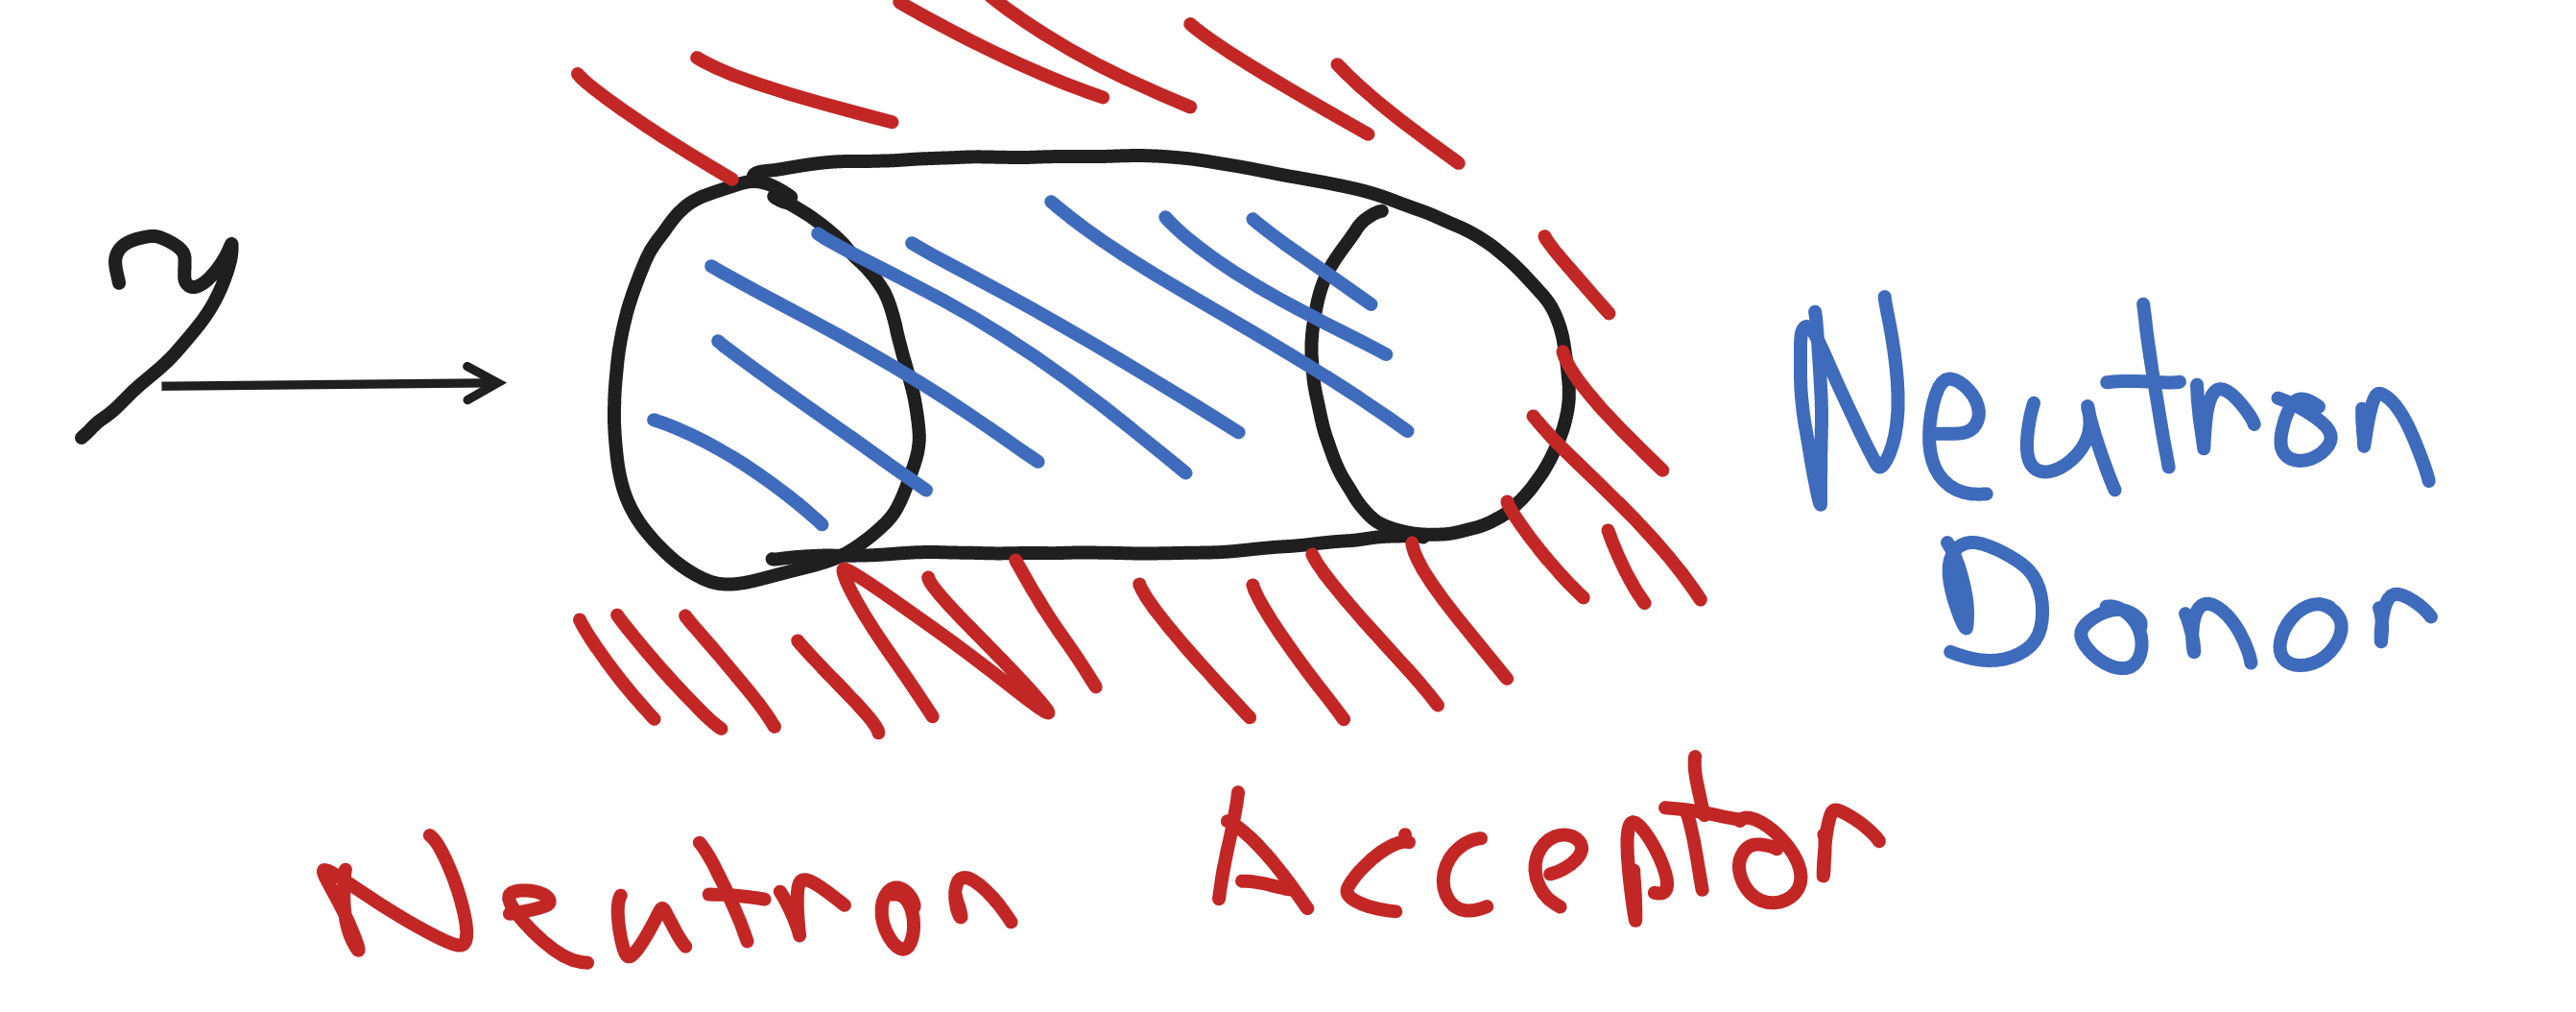
\includegraphics[scale=.4]{Images/concept setup.PNG}\\
In this setup, a gamma ray will be fired at a neutron donor (blue cylinder) which would then be captured by the neutron acceptor (red surroundings). Ideally, the neutron donor would have a very small radius but be a very long cylinder. Assuming every gamma ray produces a neutron which is then capture by the neutron acceptor, it would only cost 1 MeV/neutron with deuterium as a neutron donor (leading an energy storage efficiency of $~\frac{1}{3}$ based on the power density of decay chains work since one traverse along each chain yields $300$ keV). Can it's low cross section and density be overcome with this design? What is the ideal neutron acceptor for each neutron donor? Is this less efficient than firing protons into the neutron acceptor? 
\subsubsection{7/25/2022}
Found the readmes for the complete data libraries and found the most recent libraries \\
\subsubsection{7/26}
Doing more data wrangling using the link with the superset of all the data in the list of links file. Will combine all of the data into a singular directory for each projectile. 
\section{August}
\subsubsection{8/9/2022}
Installed and setup talys in a subdirectory of my downloads folder using WSL. In the process, I downloaded gfortran. Now have a talys executable in the bin directory of WSL. \\
Also automated and the use of the DPASS GUI to retrieve data. Takes $<$ 6 hours to retrieve the entire database. \\

\subsubsection{8/11/2022}
Made a lot more progress on the code. Wondering if radiative capture and neutron absorption are the only two competing reactions? They are certianly a subset of them. (screenshot from endf6 manual) \\
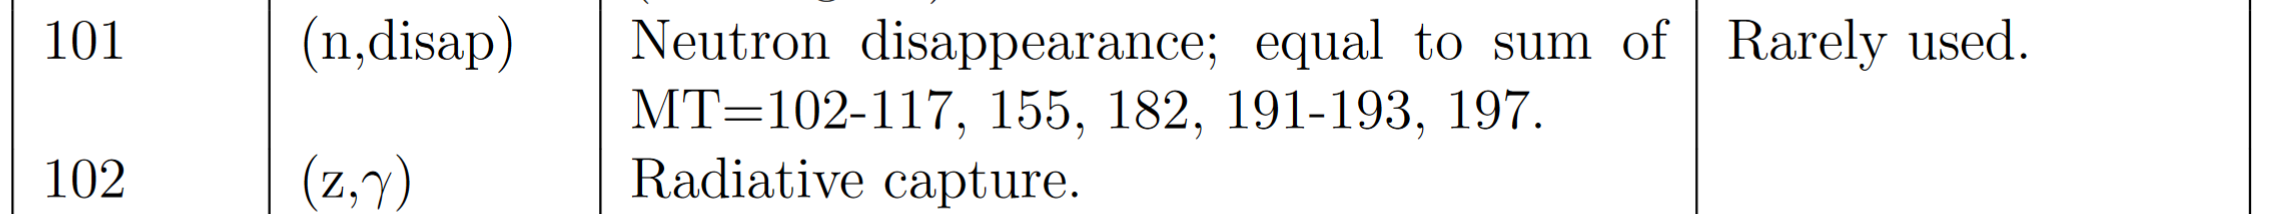
\includegraphics[scale=.4]{Images/are these the only two competing reactions.PNG}\\
I don't care about the specific reaction so much as the residual products including the desired product isotope. 

\subsubsection{8/15/2022}
Been reading \href{https://www-nds.iaea.org/exfor}{exfor} a lot recently. \\
very pleasantly surprised by some of the gamma ray cross sections of Fe-58. On the order of .001 barns at .01 MeV for the emission a neutron. We have 
\begin{equation}
    k = \frac{\rho\sigma N_A}{M}
\end{equation}
where $M$ is the molar mass in kg, $N_A$ is Avogadro's constant, $\sigma$ is the cross section in m$^2$ and $\rho$ is the mass density in kg/m$^3$. Note that for iron, $\rho N_A/M\approx 6\times10^{26}$.
Based on "On the 58Fe($\gamma$,n)57Fe reaction near a threshold" by Kitaev et al, there is a surprisingly low energy peak of 0.038 barns at 0.00597 MeV. 
$k\approx  6\sigma\times10^{26} approx  10^{-3}$. Thus, for a \textbf{thin} target it would take approximately 6 MeV to produce each neutron. Either the data is wrong or I am reading it wrong (maybe it is actually meant to be in GeV??). According to both ENDF and TENDL, it cross sections should peak at .096 barns at 19 MeV, which makes much more since when considering the nuclear binding energy that must be overcome in the $(\gamma,n)$ reaction. 
\subsubsection{August 26th}
After months of consideration I've decided on the following for my workflow: 
\begin{outline}
\1 Repetitive or computationally expensive tasks
    \2 Code these parts using the Julia language rather than Python. While I'm writing it, I can even do so in a Jupyter notebook, I just need to set the kernel to the Julia executable. There is a shortcut to do exactly this in VS code, so it is very convenient to go between kernels. 
    \2 By uploading such a notebook to Google Colab, then downloading it as a .py file, then resaving it as a .jl file, it is very fast to convert Julia Jupyter notebook into a julia script. 
    \2 \href{https://colab.research.google.com/drive/1vUglHFSJJcE75oV5qs9fQFAh6yQPVIiF?usp=sharing}{
    Example of how to run individual cells of Julia in Colab}. One can easily just call these julia scripts while invoking the Julia executable from a Python Jupyter notebook. Note that some packages are not compatible with voila and Heroku web apps, but they will work on colab as seen in the linked example. 
\1 Plots
    \2 With plotly, I can show the code how to make it on github and then put a link to where on github pages I have an interactive version of the plot :) 
\end{outline}
Honestly, one of the few things missing in Julia is Viola and the ability to easily run on heroku. Can I fix that? \\
I'm a fool and binder works with julia!!!\\
SO DOES \href{https://jupyter-tutorial.readthedocs.io/en/stable/web/dashboards/voila/index.html}{voila!! :)}
Will test this out later \\
To use Julia in binder, include a Project.toml file with the text: 
\begin{lstlisting}
[compat]
julia = "1.6"
\end{lstlisting}
The first cell should also install every package needed. \\
\href{https://github.com/MarcosP7635/binder_julia_test}{Example that works until I need to call the data}. Can I automate a backup on heroku using \href{https://binderhub.readthedocs.io/en/latest/zero-to-binderhub/index.html}{this}? \\
I really think binder is so ideal :) \\
\subsubsection{8/31/2022}
Consider a microscopic fuel cell. Whenever power is needed, a very short lived radioisotope is produced, which produces large amounts of energy.
This should allow for long shelf-life, very high specific power, and high specific energy.
Materials such a neutron reflectors seem crucial for such a reaction
\section{September}
\subsubsection{9/1/2022}
Po-208 might be one of the few isotopes with a decent energy efficiency. Consider the reactions 
Pb-208(n,p)Tl-208 and Tl-208(n,p)Po-208. This would have to be extremely fast because thallium 208 has a 3 minute half life. The decay energy of Po-208 is 5 MeV and it has half life of 3 years. \href{https://github.com/MarcosP7635/Energy/blob/main/Power_density_po_208.ipynb}{Power density calculations} Note that Po-208 undergoes alpha decay instead, so it should be calculated under the RTG.
\subsubsection{9/2/2022}
setup a firebase project in the github folder for plots \href{https://mp7635plots.web.app}{https://mp7635plots.web.app}\\
I'm considering a solenoid filled with some target that is being permeated by neutrons. In this quick drawing of a top-down view of a single loop of the solenoid, the curved black arrow represents the trajectory through the
orange target medium, and the purple sections represent electromagnets that will give the neutrons the necessary acceleration to follow this trajectory every loop. \\
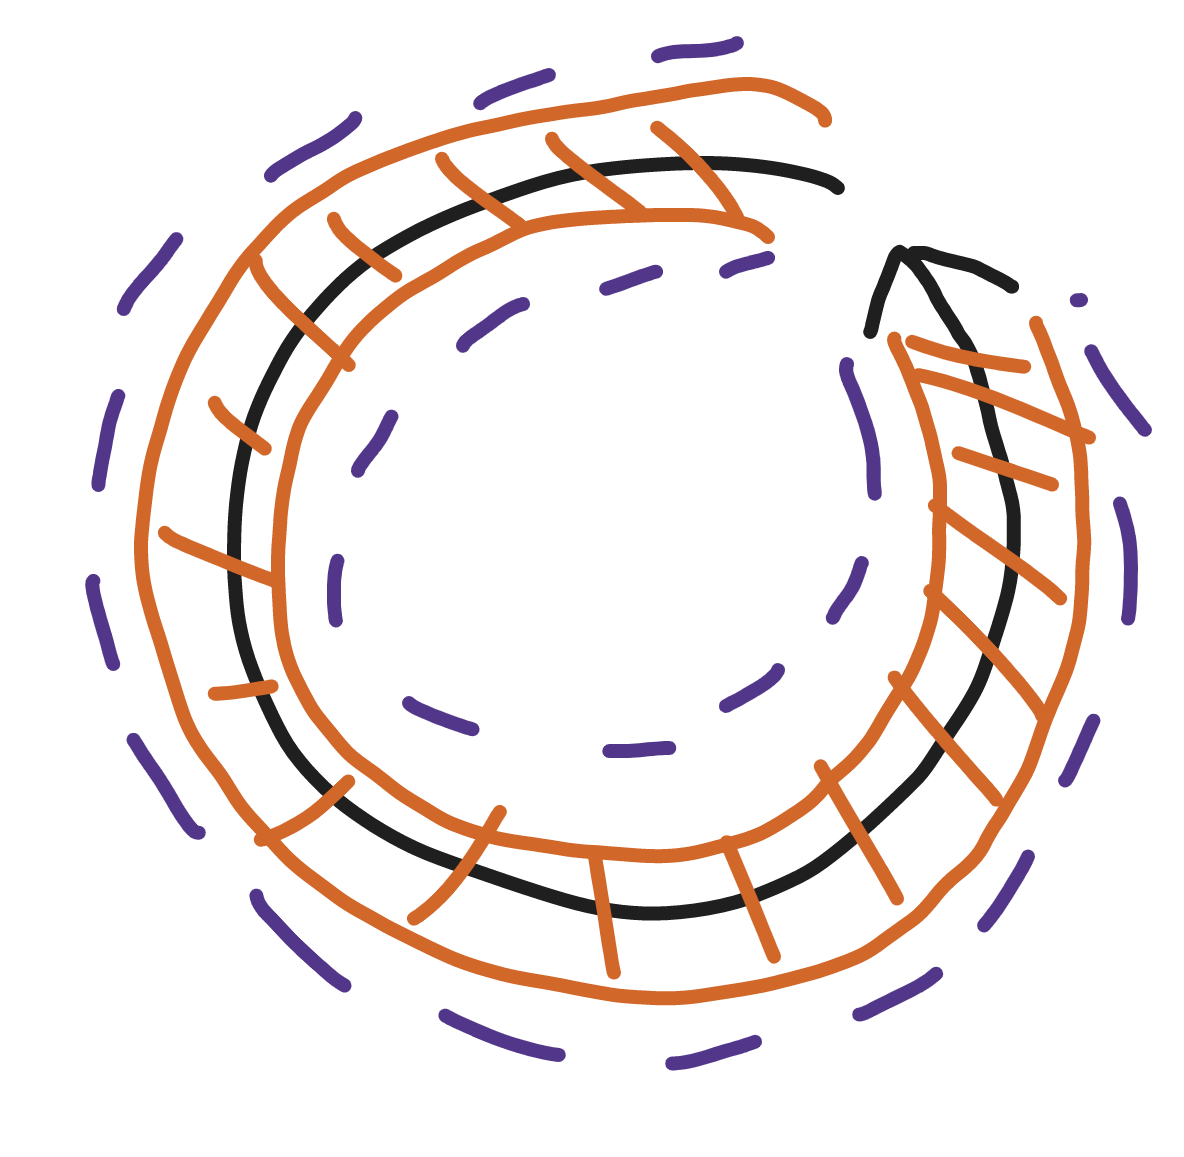
\includegraphics[]{Images/single_loop_top_down.PNG}\\
Luckily, neutrons have a non-zero magnetic moment. How much energy would such a device take, and is it better to accelerate protons instead? The purpose of using a solenoid is to allow the neutron to travel a large distance within the target medium to account for a small reaction cross section. Furthermore,the solenoid design allows the experiment to not take up a large volume for potentially km-scale travel distances. \\
Is it possible to make the neutron follow this trajectory with a singular magnetic field that works to similarly to a gravitational field? 
\subsubsection{9/6/2022}
LADWP serves 1200 km2 of area. 
it would take 10$^{10-1.5}$ = 10$^{8.5}$ m$^2$ = 300 km$^2$ of solar panels to power LA. So LA needs to cover 1/3 of the county in solar\\
Checked using google earth and solargis. \\
\includegraphics[scale=.62]{Images/solar irradiance la county screenshot.PNG}\\
\includegraphics[scale=.62]{Images/solar irradiance sf valley screenshot.PNG}
\subsubsection{9/7/2022}
If energy can be efficiently recovered from $\gamma$ rays by heating up a thick shielding, which is then connected to a thermocouple, then the following may be an energy efficient way of producing neutrons\\
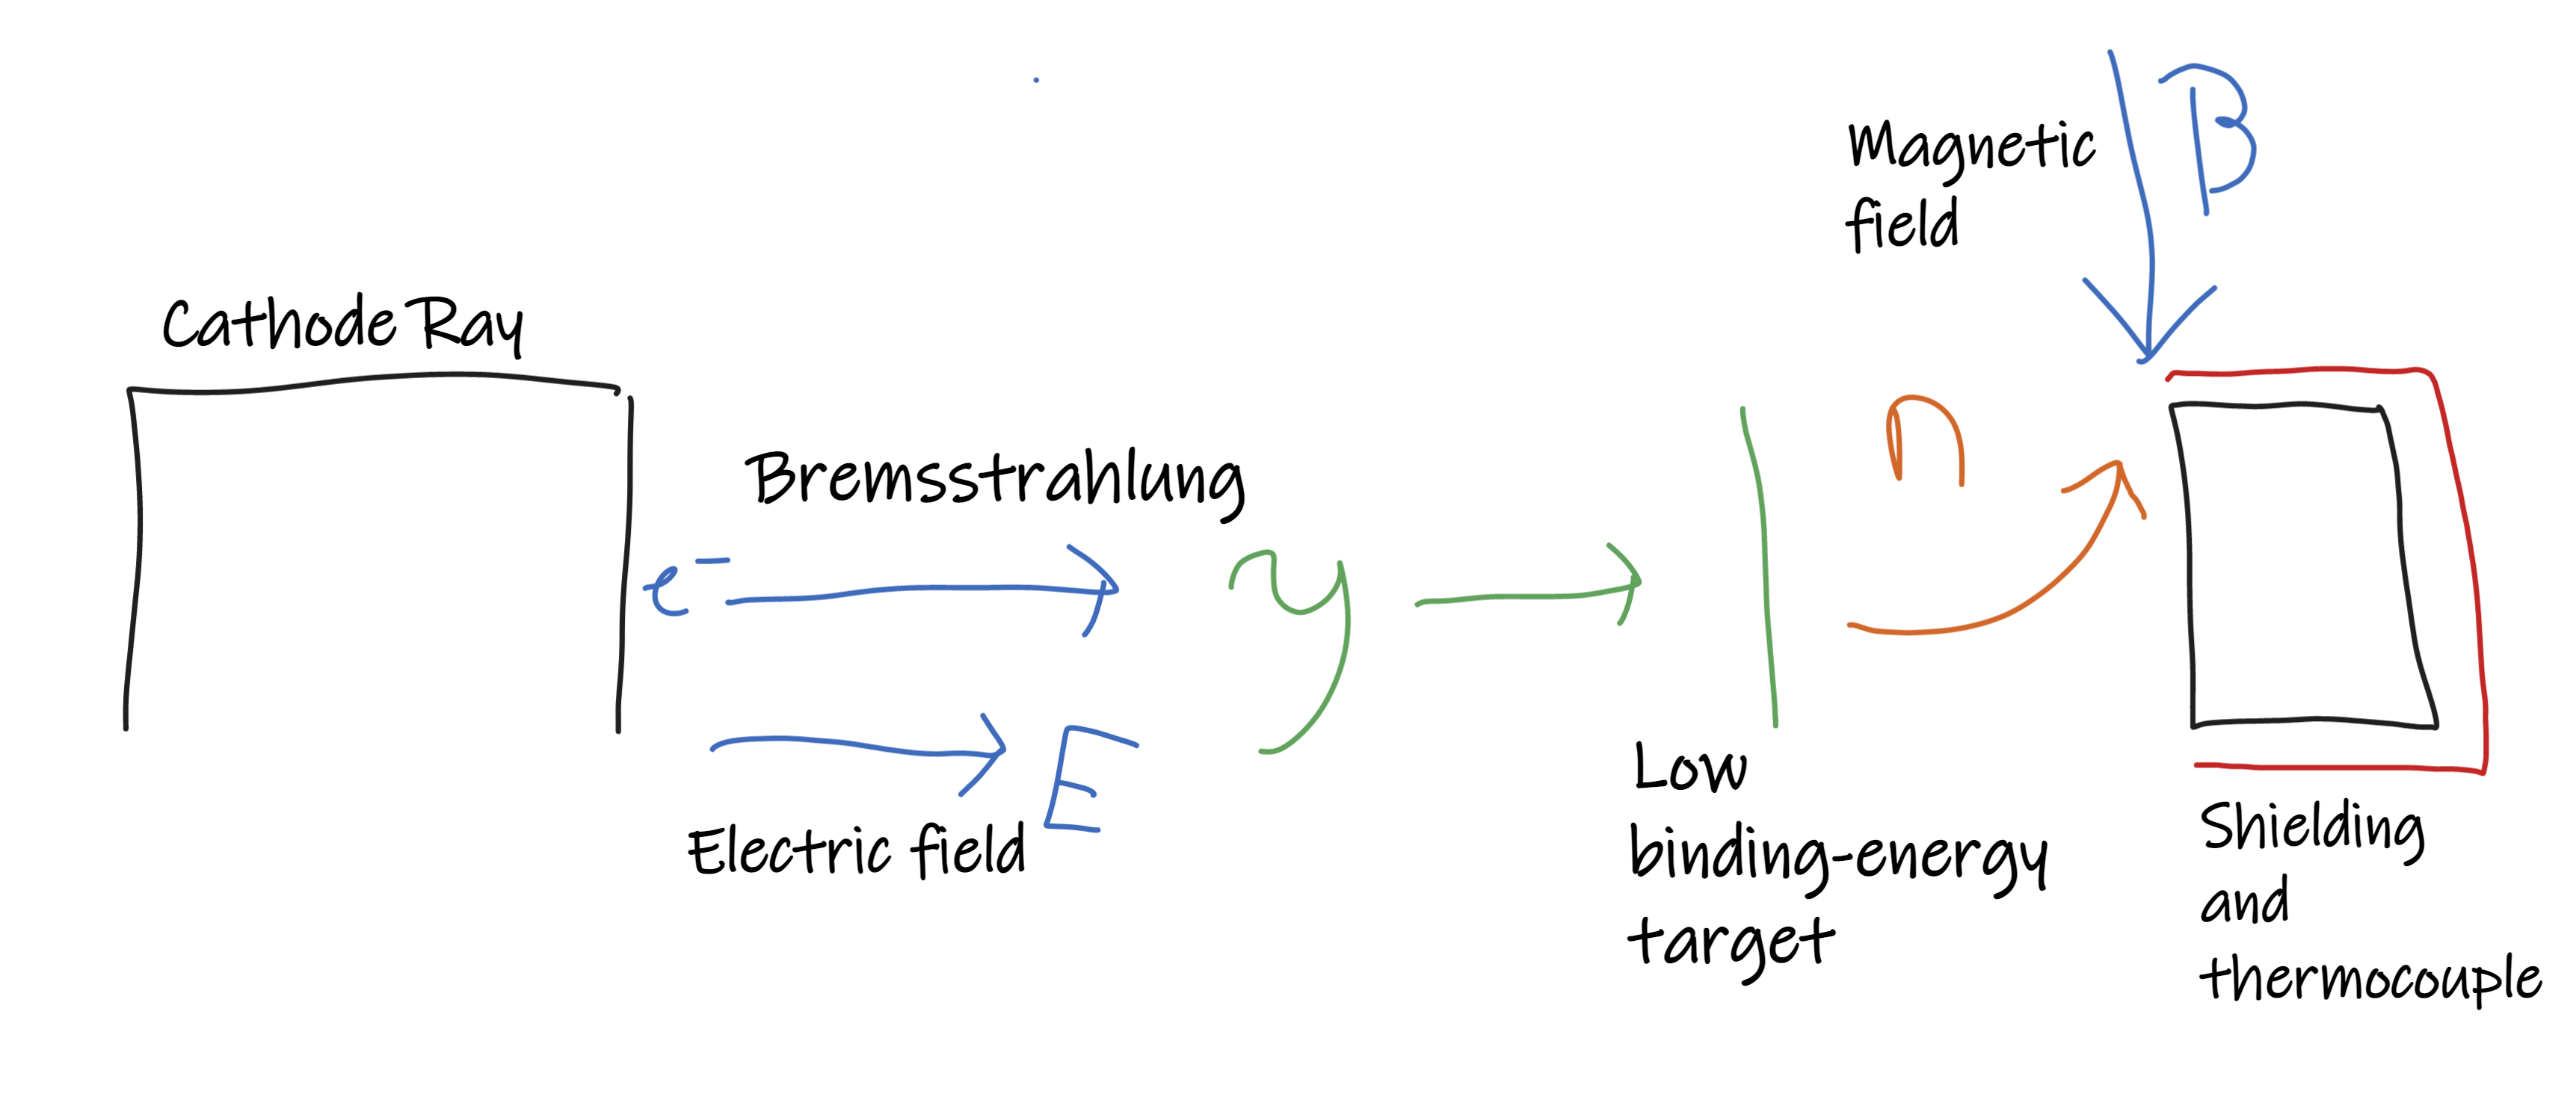
\includegraphics[scale=.65]{Images/neutron generator concept.PNG}\\
\subsubsection{9/12/2022}
Thought of a new setup for generating radioisotopes. This prioritizes energy efficiency by making use of spallation by relativistic protons. These protons are accelerated using the wake field of a plasma, which is created with laser. 
The spallation of protons onto the target releases neutrons which are then guided by a magnetic field to make many loops through a circular target to ensure a reaction. See the zotero group for more information on spallation, lasers, and neutron interactions through matter and magnetic fields. \\
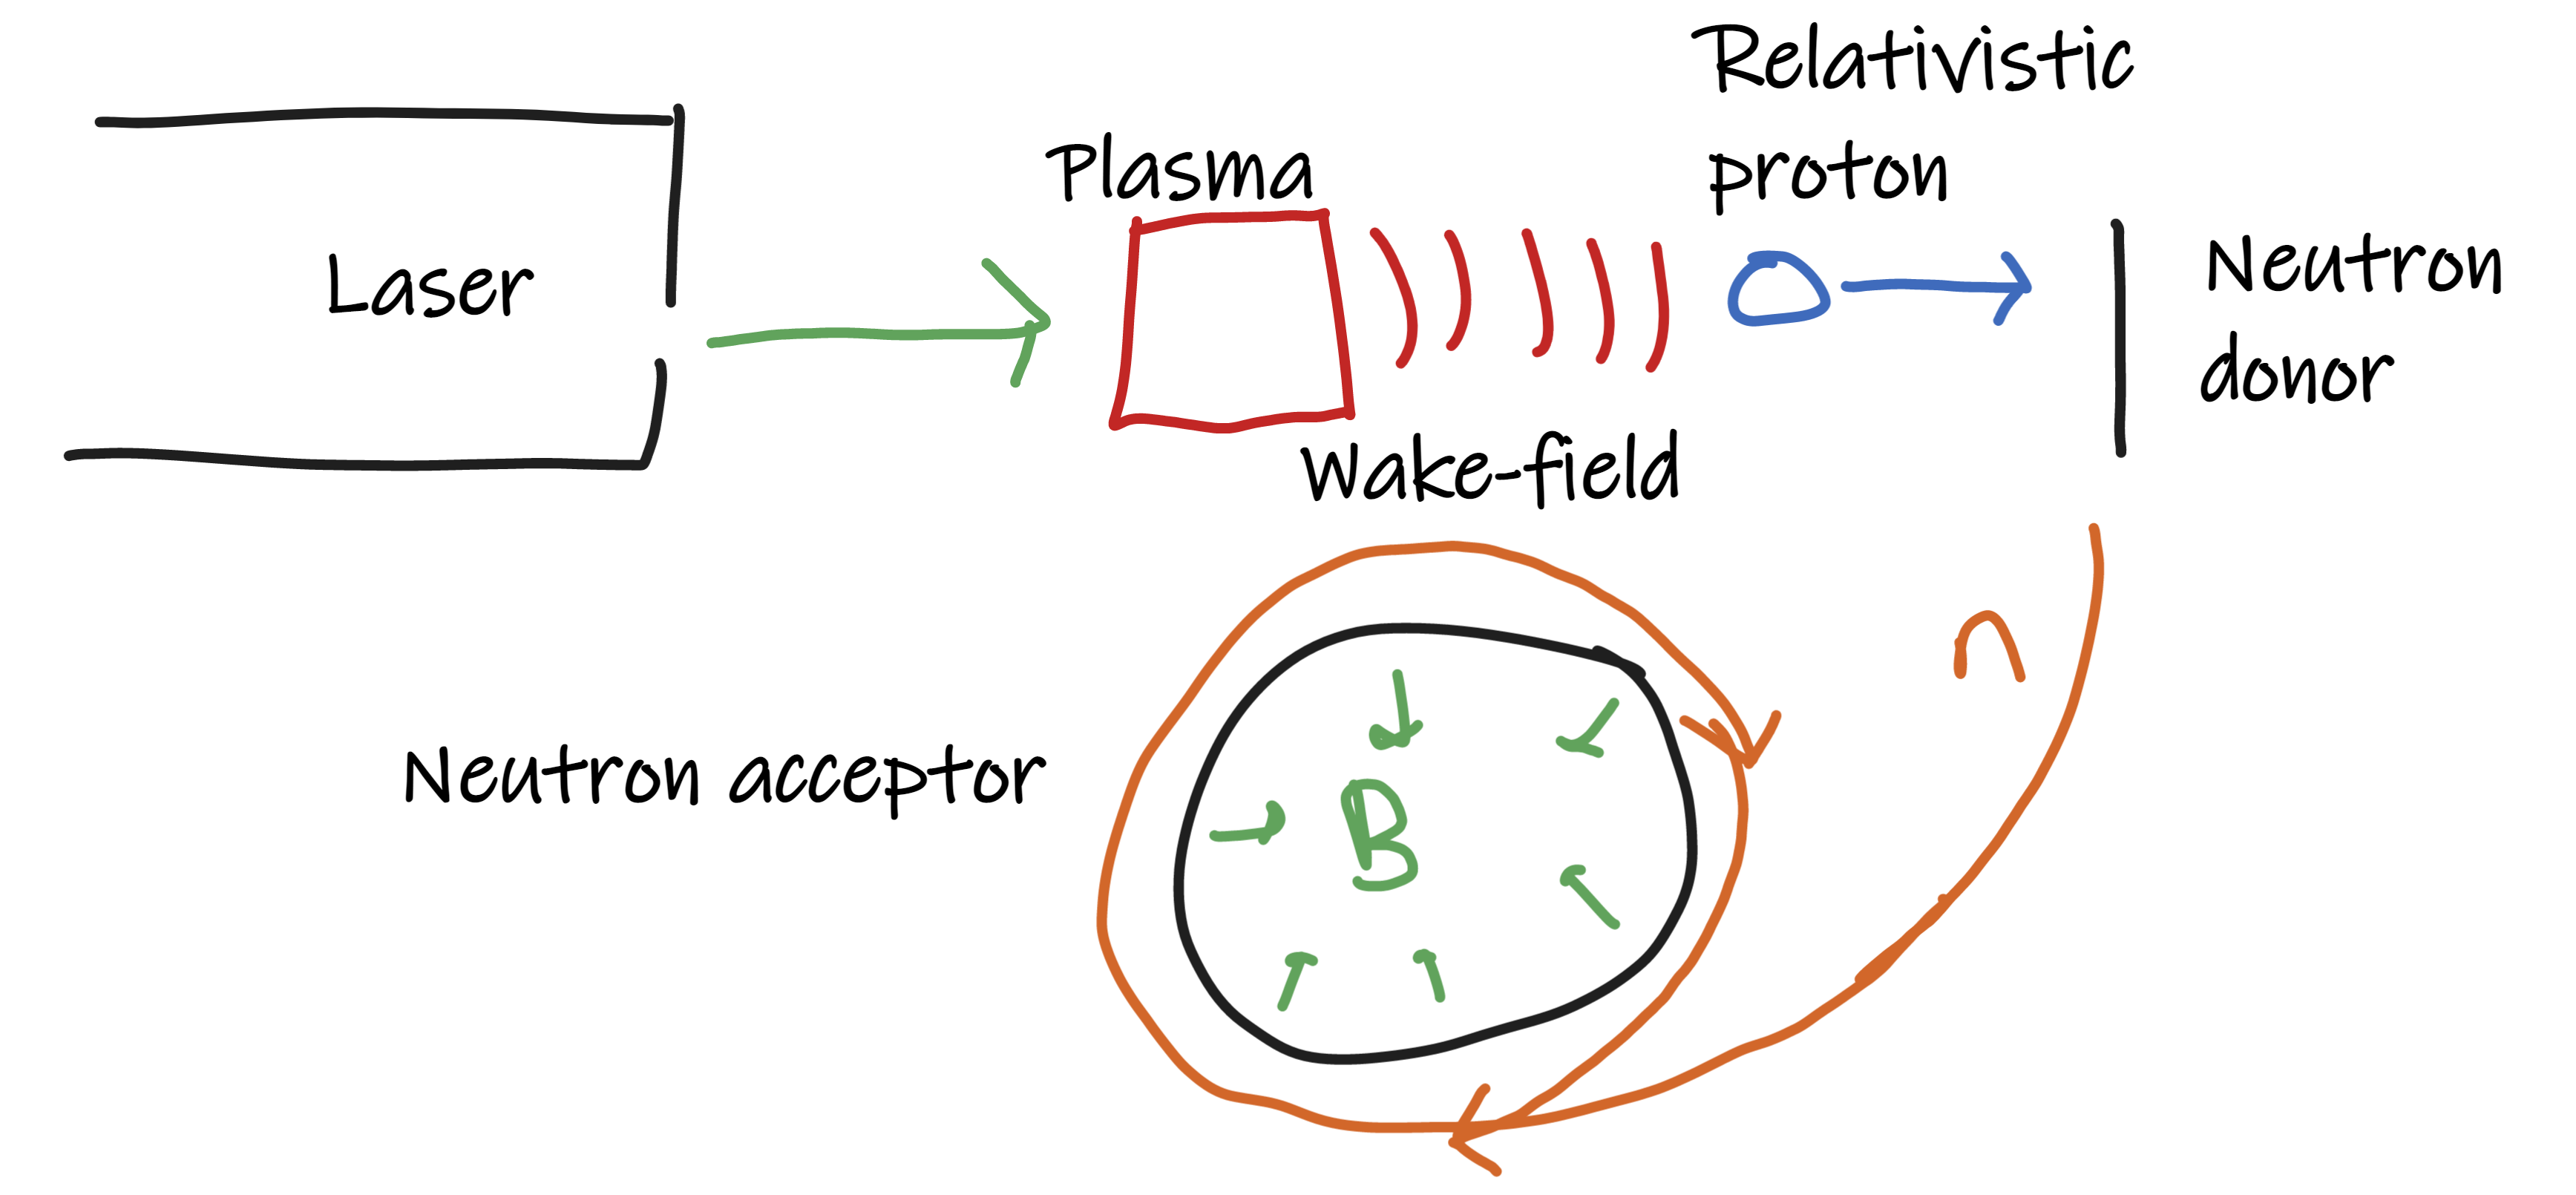
\includegraphics[scale=.65]{Images/laser plasma accelerated spallation neutron generator concept.PNG}\\
Note that a magnetic field guides the neutron through the target. \\
Now to simulate this setup. I'll call it laser plasma wakefield spallation neutron source (LPWFSNS) 
\subsubsection{9/13/2022}
Most plamsa wakefield accelerators are designed to accelerate electrons rather than protons. However, I wonder if energy efficient acceleration of protons can also be achieved. \href{http://dx.doi.org/10.1098/rsta.2019.0215}{Hidding et al. RSP. 2019} claim that separating electrons and ions within a plasma can generate electric fields on the order of TV/m, and that intense laser pulses or particles are sufficient energy sources. 
\subsubsection{9/14/2022}
Mostly reading papers on proton accelerators and calculated their energy efficiency. Accelerating a protons using an electron beam such as those produced by laser wake field particle accelerators (LWFPA) is 1000x more efficient than currently existing neutron generators. However, this would still be $<$1\% energy efficient for energy storage. \\
Consider a much simpler case, using brehmsstrahlung of electrons to produce gamma rays. The cross section of the reaction $^2$H(g,n)$ ^1$H is on the order of 10$^-2.5$b $= 10^{-30.5}$m$^2$ for 4.5 MeV $\gamma$ rays. We have for the probability of the reaction 
\begin{equation}
\begin{split}
\\
\end{split}
\end{equation}
\subsubsection{9/15/2022}
I should take into greater account the energy consumed and produced in nuclear reactions. \\
Would stripping all of the electrons from an atom that can only decay by electron capture stop it from decaying? If so, this seems like an effective way to control the decay radioisotopes.\\
From the Rydberg formula, an atom's ionization energy is proportional to $Z^2$. This gives a maximum of 13,000x larger than hydrogen's ionization energy of 13 eV. This assumes that all electrons are held at the same radii, which they aren't. 
Found some ionization energies here: https://webbook.nist.gov/chemistry/ie-ser/ and https://physics.nist.gov/PhysRefData/ASD/ionEnergy.html and https://physics.nist.gov/cgi-bin/ASD/ie.pl in case I need them later. 
\subsubsection{9/16/2022}
How many decay chains can use electron capture as a stopping point? Ideally, they would then decay into an isotope that quickly releases a lot of energy. Fully ionizing such a nucleus seems like an interesting way to pause a decay chain. Are there other ways of achieving this without relativistic effects? 
\subsubsection{9/17/2022}
What is the energy efficiency of use neutrons travelling in a circle to cause the reaction $^2$H(n,2n) \href{https://www-nds.iaea.org/dataexplorer/?target_elem=H&target_mass=2&reaction=n\%2C2n}{link on data explorer}.\\
\href{https://www-nds.iaea.org/dataexplorer/?target_elem=H&target_mass=2&reaction=n\%2Ctotal}{total neutron cross sections for deuterium on data explorer}
\subsubsection{9/18/2022}
Trying talys because my brain hurts. Some of the ENDF reaction cross sections are larger than their corresponding total cross sections. By definition, that reaction cross section is part of the sum equal to the total cross sections. That means there is a negative cross section of a different reaction at that energy and/or something is very wrong. \\
Saved the results in a file named verify\_ouput.txt\\
Tests passed: 20526\\Tests failed: 2084\\Tests failed and ignored: 192
\subsubsection{9/19/2022}
Is the violation of the summation rule the result of multiple reactions happening per projectile in the model??
\subsubsection{9/22/2022}
Maybe I'm just not taking into account multiplicity? When I run the talys command line tool, that is one of the outputs. What does that mean here? Is that the average number of reactions per cross section? The smallest element the command line tool will work with is lithium :/. \\
In section 4.2.4 page 71 of "TALYS-1.96/2.0
Simulation of nuclear reactions" by Arjan Koning, Stephane Hilaire, and Stephane Goriely, the neutron multiplicity $Y_n$ is defined as 
\begin{equation}
\begin{split}
Y_n = \frac{\sigma_n}{\sigma_{non-el}}\\
\end{split}
\end{equation}
where $\sigma_n$ is the total neutron production cross section and $\sigma_{non-el}$ is the nonelastic collision cross section. In more detail, the total neutron production cross section is defined as 
\begin{equation}
\begin{split}
\sigma_n = \sum_{i_n=0}^\infty\sum_{i_d=0}^\infty\sum_{i_p=0}^\infty\sum_{i_t=0}^\infty\sum_{i_h=0}^\infty\sum_{i_\alpha=0}^\infty i_n\sigma^{ex}\
\end{split}
\end{equation}
where $i_x$ is the number of outgoing particles named $x$ ($i_n$ is the number of outgoing neutrons) and $\sigma_{ex}$ is a cross section specific to a given number of outgoing particles. Thus, the number I have been looking for is actually $\sigma_{ex}$ not $\sigma_n$! 
\subsubsection{9/23/2022}
Another advantage of pushing interactive html to my plots github repo is that it also shows up on firebase.  \href{https://mp7635plots.web.app/avg_b_energy_vs_half_life.html}{E.g.}
\subsubsection{9/24/2022}
There are 49 sub-directories in ENDF-libraries. My main goal right now is two-fold: find what naturally occurring isotopes are ideal for spending the least amount of energy to produce neutrons by accelerating neutrons through the material; and finding what decay chains are ideal to quickly produce electricity. For working energy storage in space or underwater, the ideal decay chain also produces the original neutron source and target.
\subsubsection{9/25/2022}
I found out what data was being used from tendl on the data explorer website, so I programmatically downloaded that over the course of an hour from google colab in julia :) \\
Backed up the Jupyter notebook where I did so in my github repo :)\\
I think this data actually follows the summation rules so that is a good sign.\\
Just plotted the average binding energy per nucleon vs. energy required per neutron produced using a perfectly efficient neutron accelerator. The best neutron source for the target of such a neutron accelerator is 9Be. The theoretical maximum is approximately 0.06 neutrons per MeV. Deuterium was .014 neutrons per MeV. They appear to be directly improportional, but only for the top right region of the graph. Why does the rest seem to not follow the same relationship? 
\subsubsection{9/26/2022}
Inverted the y-axis on the plot and made this\\
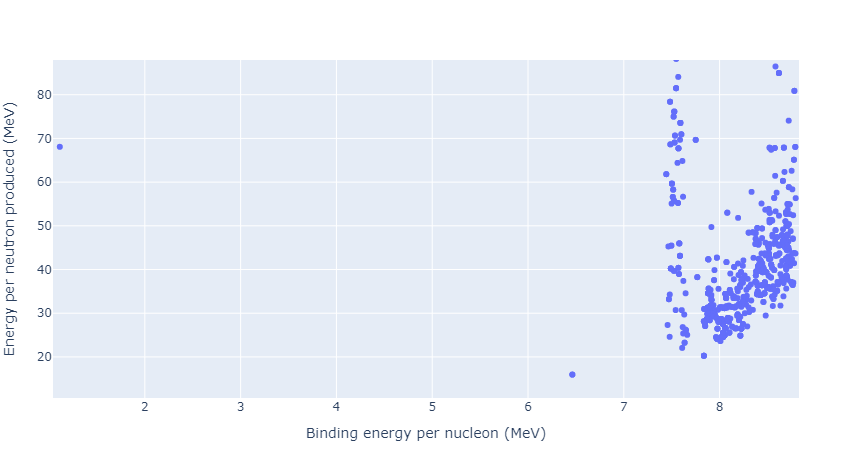
\includegraphics[scale=.6]{Images/binding_energy_vs_energy_per_neutron.png}\\
The far off-left points are deuterium and beryllium-9, respectively. 
\subsubsection{9/27/2022}
Redid all of the power density time series calculations for all of the beta decay chains. It was much faster when I rewrote it in Julia (only takes 4 minutes vs. the hour it took in Python). The minimum energy to produce neutrons I calculated does not take into account the kinetic energy of the incident and produced neutrons. How accurate of an approximation is the Q-value?
\subsubsection{9/28/2022}
Between 20,000 and 100,000 seconds, the Pb212 decay chain has a specific power of 10 MW / mole, so this would be very useful for solar farms. At the 10$^6$ seconds (two weeks) 223 Ra produces 300 kw / mole. \\
The decays subdirectory of ENDF8 lists the average decay data for a number of nuclides. I can also use JENDL-5 and JEFF 3.3 (ENDF libraries-2). Now I can build new decay chains using the average decay energy for all decay types :) 
\subsubsection{9/30/2022}
jendl5 has B+/EC average energy and jeff33 has average spontaneous fission energies
\section{October}
\subsubsection{10/1/2022}
Made a very user-friendly colab notebook to plot the specific power of a given isotope and it works :) \\
Need to check why some isotopes (such as Bi-207) have 0. Is it because they're not in livechart?\\
For isotopes with multiple decay modes, do the different decay modes have different half lives?
\subsubsection{10/2/2022}
Can now account for electron capture. \\
The maximum power densities are now very different now that I actually use the average decay energy rather than the maximum. \\
I should be more specific in what I mean by "power produced". I could just take the average kinetic energy of the be\\
Apparently ENDF8 has more data than everything else. \\
I can just add the sum of the energies, excluding the neutrino energy from endf8. \\
\href{tinyurl.com/power-density-viewer}{tinyurl.com/power-density-viewer}\\
3 kg of Na-24 can power an airplane continuously for an entire day. 
\subsubsection{10/3/2022}
I overestimated power time series because I count the earlier decay steps an additional time for each decay mode beyond the first. How do I prevent this? 
I can rewrite the function power\_per\_mole to account for this. 
\subsubsection{10/4/2022}
Writing a function to prevent the overestimate. Comparing strings in nested vectors is very slow, and managing trees is beyond the scope of this project (and my time and energy). Thus, I'll just generate the decay chains as needed rather than drawing from a CSV or dictionary.\\
Representing decay chains as a dictionary is by far the cleanest and simplest solution.  \\
The dictionary method doesn't work because different steps could have the same decay energy. Nested dictionaries, however, should work. 
\subsubsection{10/5/2022}
Nested dictionaries do work. I realize I can have one big dictionary storing the decay info of every isotope. To make the decay chain of a given isotope, I just make a different dictionary where the parent is the decay of the given isotope. \\
For the half lives and decay modes should I exclusively use ENDF8? 
\subsubsection{10/8/2022}
Some quick OOM. Assuming a neutron's magnetic moment is aligned with a magnetic field, we have for the force experienced by the neutron where $m_n$ is the mass of the neutron, it is moving at a velocity $v$, and it is moving in a circular path with a radius $r$
\begin{equation}
\begin{split}
F= \frac{m_nv^2}{r} = s\nabla B\\
v = \sqrt{\frac{rs\nabla B}{m}}\\
\end{split}
\end{equation}
According to \href{https://doi.org/10.1063/1.3664092}{Zanini et al. APL. 2011.},
micro magnet arrays can achieve magnetic field gradients on the order of $10^6$T/m. Thus we have for the velocity of neutrons on the track $\log_{10}v = \frac{1}{2}(-1 - 26 + 6 + 27) = 3$. Thus this should be able keep neutrons on a circular path for kinetic energies $\log_{10}T = -27 + 6 = -21$ or .01 eV. For thermal neutrons, the gradient of the magnetic field would need to be on the order of $10^7$T/m. Of course, a larger radius of 1 m would also be sufficient.
\subsubsection{10/9/2022}
Is deuterium tritium fusion practical yet? If so, making tritium would be a great way to store energy. What is the specific energy of tritium deuterium fusion? 17.6 MeV per reaction $\approx10^7$MeV$\approx10^{-12}$J. Per mole of reaction this is approximately $6\times10^{11}$. Each mole will have approximately 5 grams of mass so this gives $\approx10^{11}$J/g. At STP, hydrogen has a density of $\approx10^{-1}$kg/m$^3$, and thus we have a power density of $\approx10^{13}$J/m$^3$ or $\approx10^{10}$J/L. Gasoline only has a specific energy of $<10^8$MJ/kg and an energy density of $<10^8$J/L. No it isn't practical yet. \\
\subsubsection{10/10/2022}
Can I make a particle go through loops using the coriolis force? For a frame rotating at an angular velocity $\omega$, and a particle moving within that frame at a velocity $v'$ the resulting acceleration from the coriolis force is $-2(\omega\times v')$. By definition, if the reference frame is rotating with radius $r$ and velocity $v$, and assuming all angles are normal 
\begin{equation}
\begin{split}
a_{coriolis} = -2(\frac{v}{r})\times v' = \frac{v'^2}{r'}\\
r' = \frac{v'r}{-2(v)}
\end{split}
\end{equation}
Assuming we want this circle within the rotating frame to stay within the radius $r$
\begin{equation}
\begin{split}
2r' < r\\
\frac{v'r}{v} < r\\
v' < v\\
\end{split}
\end{equation}
\subsubsection{10/14/2022}
Example of a decay chain I was able to display programmatically :)\\
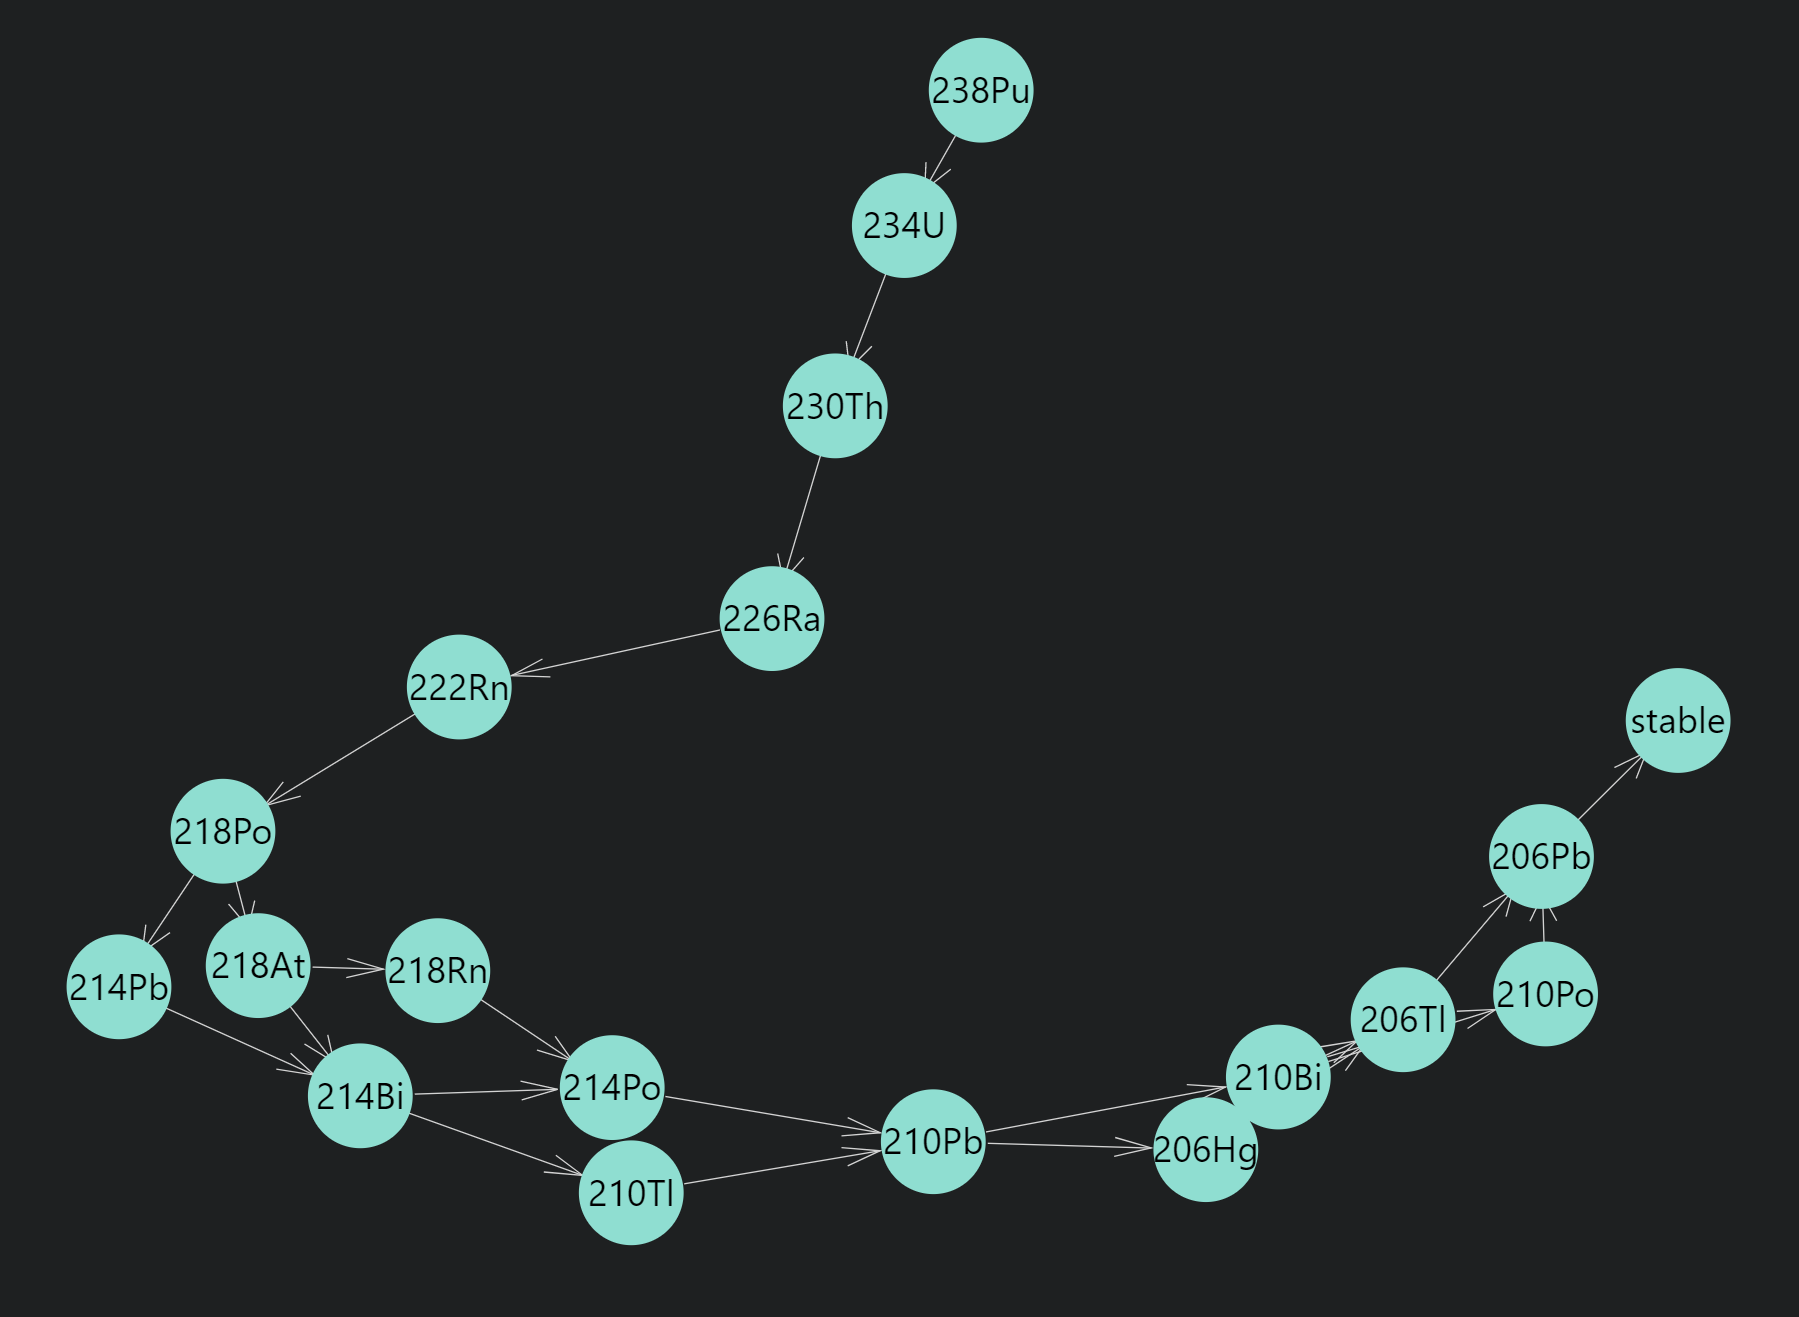
\includegraphics[]{Images/better_snip.PNG}
\subsubsection{10/17/2022}
After spending a lot of time debugging, I've been able to calculate the power contribution of an isotope to its decay chain. Consequently, the total power produced by a decay chain as a function of time. Additionally, future work will incorporate the type of energy and the spectra of the radiation produced. This is in the Jupyter notebook named 
\begin{verbatim}
    make_comprehensive_power.ipynb
\end{verbatim}
which runs Julia. When simulating just the power output, each time step for all approximately 2,500 decay chains takes about 3 seconds on my laptop. \\
I have not been taking the annihilation of positrons from beta+ decay into account. \\
Success! Now my value for the specific power of plutonium matches that used for RTGs :) (0.55 W/g). \\
Made this: new colab notebook to plot data interactively in list of links. 
\subsubsection{10/18/2022}
trying nbinteract to make a webpage. some of the dependencies don't work. sticking with colab. might make interactive plotly export. \\
It works on streamlit! :) \\
https://marcosp7635-power-densities-plot-power-de1e9n.streamlitapp.com/\\
woohoo! :)\\
Also this: \href{https://tinyurl.com/plot-isotope-power}{https://tinyurl.com/plot-isotope-power}\\
I should find the total energy in each decay chain and the time where the decay produces the most energy. \\
Make a new website that gives a ranking of the isotopes for a given time range of power. 
\subsubsection{10/19/2022}
It's possible for me to put entire projects on interactive websites using streamlit, colab, and binder.\\
\subsubsection{10/26/2022}
How do I visualize the energy produced by different decay chains as a function of time? I'll just plot them for now. 
\subsubsection{10/27/2022}
Made this \\
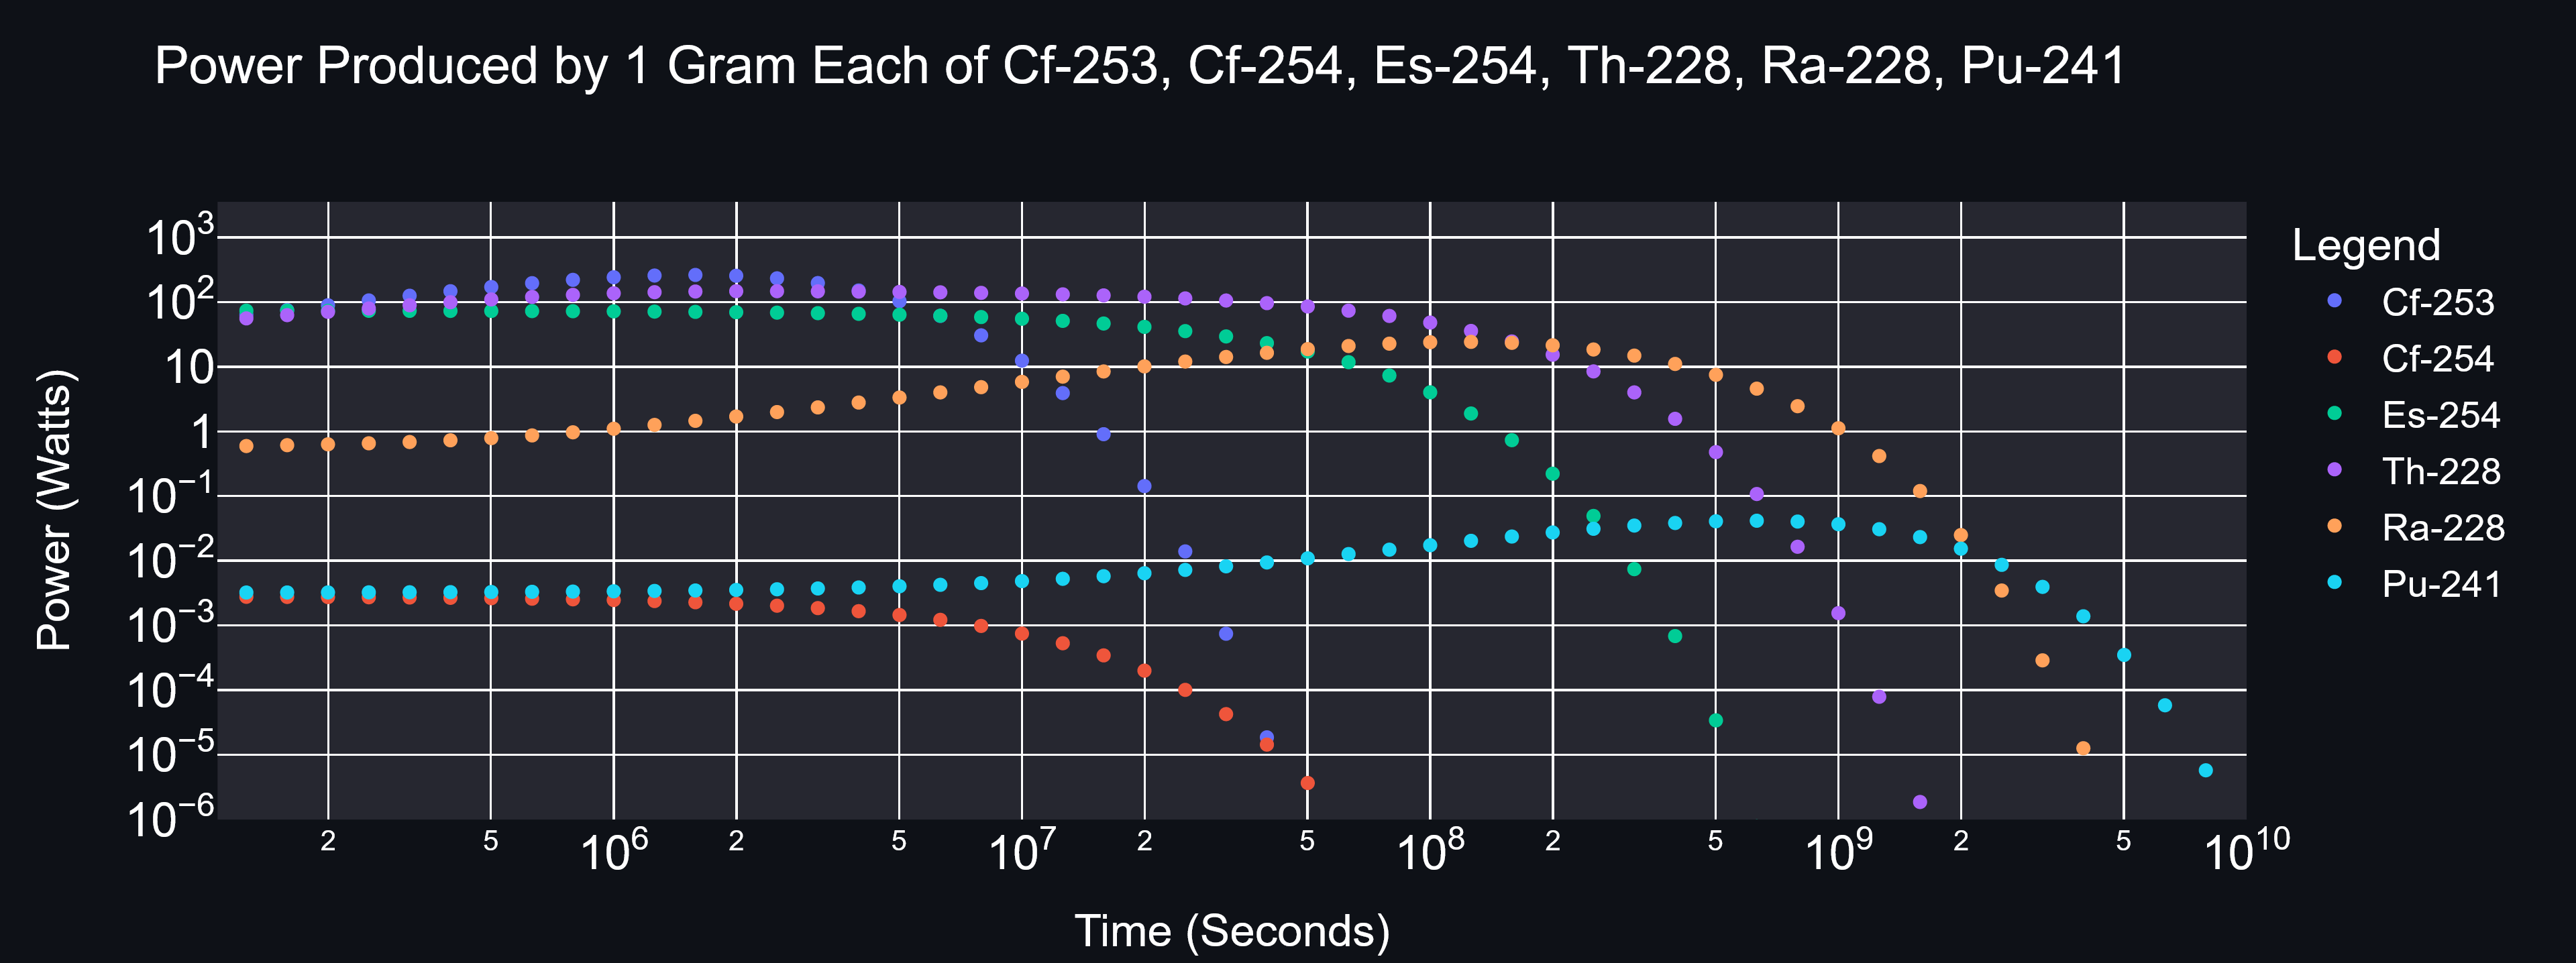
\includegraphics[scale=.6]{Images/example_plot.PNG}
\subsubsection{10/30/2022}
Since I have already downloaded lots of data for the cross sections of numerous nuclear reactions, I can use AMU2020 to calculate the q-value for each of these reactions. Additionally, I have already calculated the energy produced by different decay chains of radioisotopes. Thus I can evaluate the energy efficiency of each of these reactions. \\
\textbf{Action items:}
\begin{itemize}
    \item Calculate the q-value for every nuclear reaction, and how much energy each reaction requires. 
    \item Find all of the corresponding ways to release energy for every nuclear reaction. Make sure that these can happen on-demand rather than passively. Accidentally releasing the energy stored is unsafe, and would make the storage pointless. 
\end{itemize}
\section{November}
\subsubsection{11/7/2022}
to move forward with the simulations, only consider 1 step reactions. For the efficiency, neutrons can use the ratio of the reaction cross section to the total cross section. The actual probability will have to be calculated for charged particles.

\subsubsection{11/8/2022}
Running into the same problem from before when the total cross section is less than one of the reaction cross sections. Maybe this is why? This excerpt is from Section 2.4.9 in the ENDF Manual and page 84. 
\begin{lstlisting}[breaklines]
To avoid negative cross sections, new evaluations should use only the rigorous formulations
such as Reich-Moore (LRF=3) or R-Matrix Limited (LRF=7). However, resonance param-
eters coded in other formats may be encountered in some old evaluations.
\end{lstlisting}
Checking if the data stored in the data explorer has the same problem. 
Have a directory in the imported data directory named \begin{verbatim}
    tendl_total_neutron_sigma_data
\end{verbatim}
where I have already stored some of the neutron cross sections and a script to get them. It is intended to be run on colab. The relevant jupyter notebook is named \begin{verbatim}
    automating_data_explorer.ipynb
\end{verbatim}
Also here is the format of the open in colab button written in markdown that you can just add to any notebook on github. 
\begin{lstlisting}[breaklines]
<a href="https://colab.research.google.com/github/MarcosP7635/Energy/blob/main/JupyterNotebooks/automating_data_explorer.ipynb" target="_parent"><img src="https://colab.research.google.com/assets/colab-badge.svg" alt="Open In Colab"/></a>
\end{lstlisting}
I should go through all of the data I have to figure out what datasets have this problem. 
\subsubsection{11/8/2022}
Create a web app where you enter the use case and the app returns the appropriate radioisotopes, conversion method, shielding required, msds, and how to produce it (and who currently does it)
\subsubsection{11/13/2022}
Added a new plot to the web app and took this screenshot of me using my streamlit app. \\
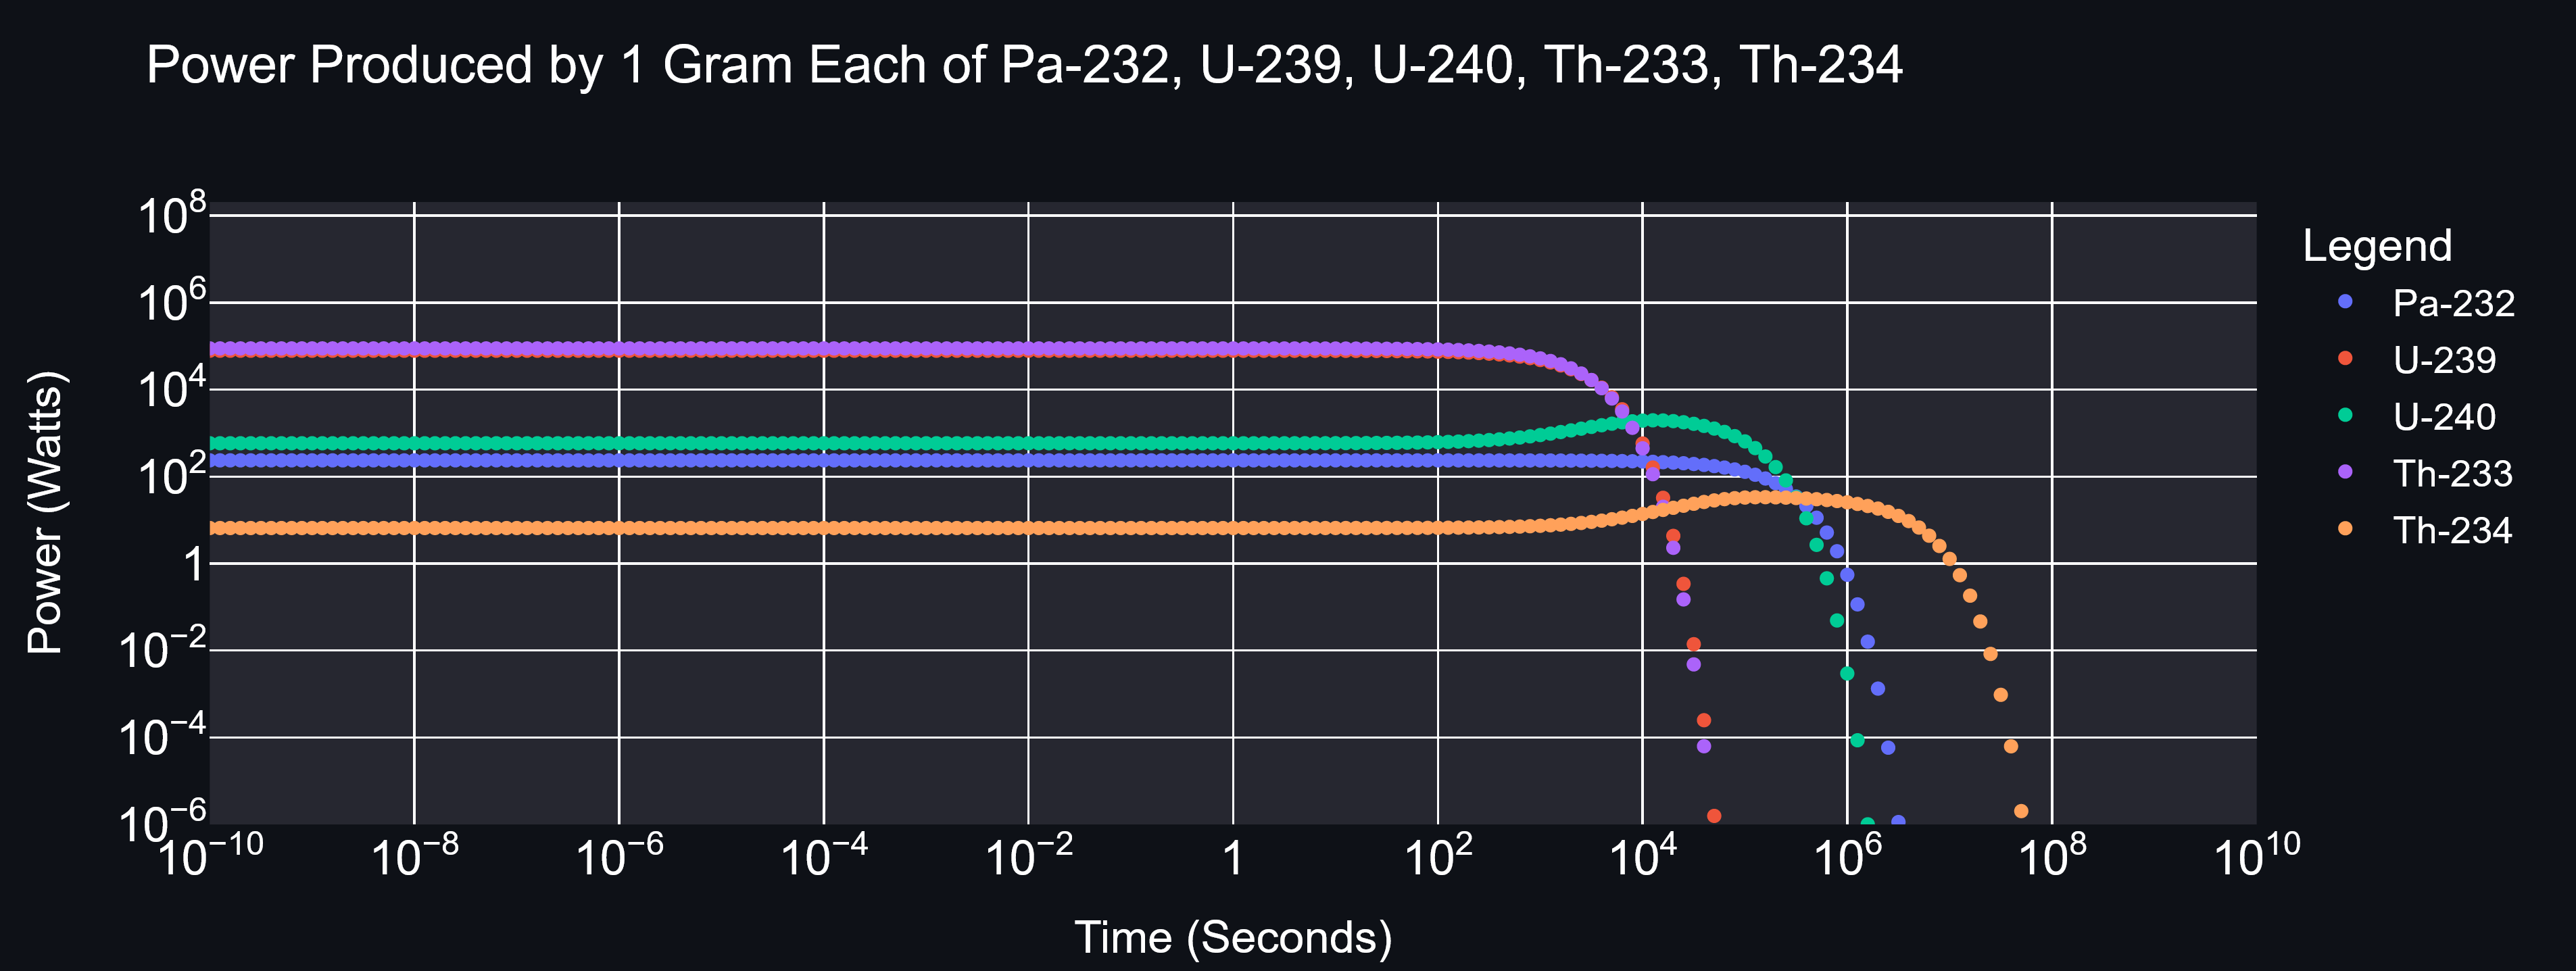
\includegraphics[scale=.6]{Images/newplot(4).png}\\
This does not take into account the efficiency of converting this power into electricity, and it does not account for the fraction of neutrons that would be absorbed the target nucleus. These isotopes were selected because they can, at least in theory, be produced by irradiating a naturally occurring isotope and the total energy release during their decay is more than the minimum energy it would take to produce these neutrons (~ 16 MeV / neutron). See either of these interactive plots for the efficiencies of other isotopes: \href{https://marcosp7635.github.io/plots/keV_per_neutron.html}{github pages version} and \href{https://mp7635plots.web.app/keV_per_neutron.html}{firebase version}. Neither of these plots include parent isotopes that have less neutrons than the naturally occurring isotopes of the same element. 
\subsubsection{11/15/2022}
What if we were deliberate about the path and target of individual beta particles (or alpha particles or gamma rays, etc.) and how each one was converted into electricity? What if we could use the same technology that embeds transistors onto a silicon chip to embed radioisotopes into a conversion setup, something more efficient and direct than the Seebeck effect. On the smallest scale, what can we use to catch radiation and use it to drive electrons? Or have radiation interfere with some target structure. 
\subsubsection{11/18/2022}
What kind of shielding would you need for using these isotopes to store energy?\\
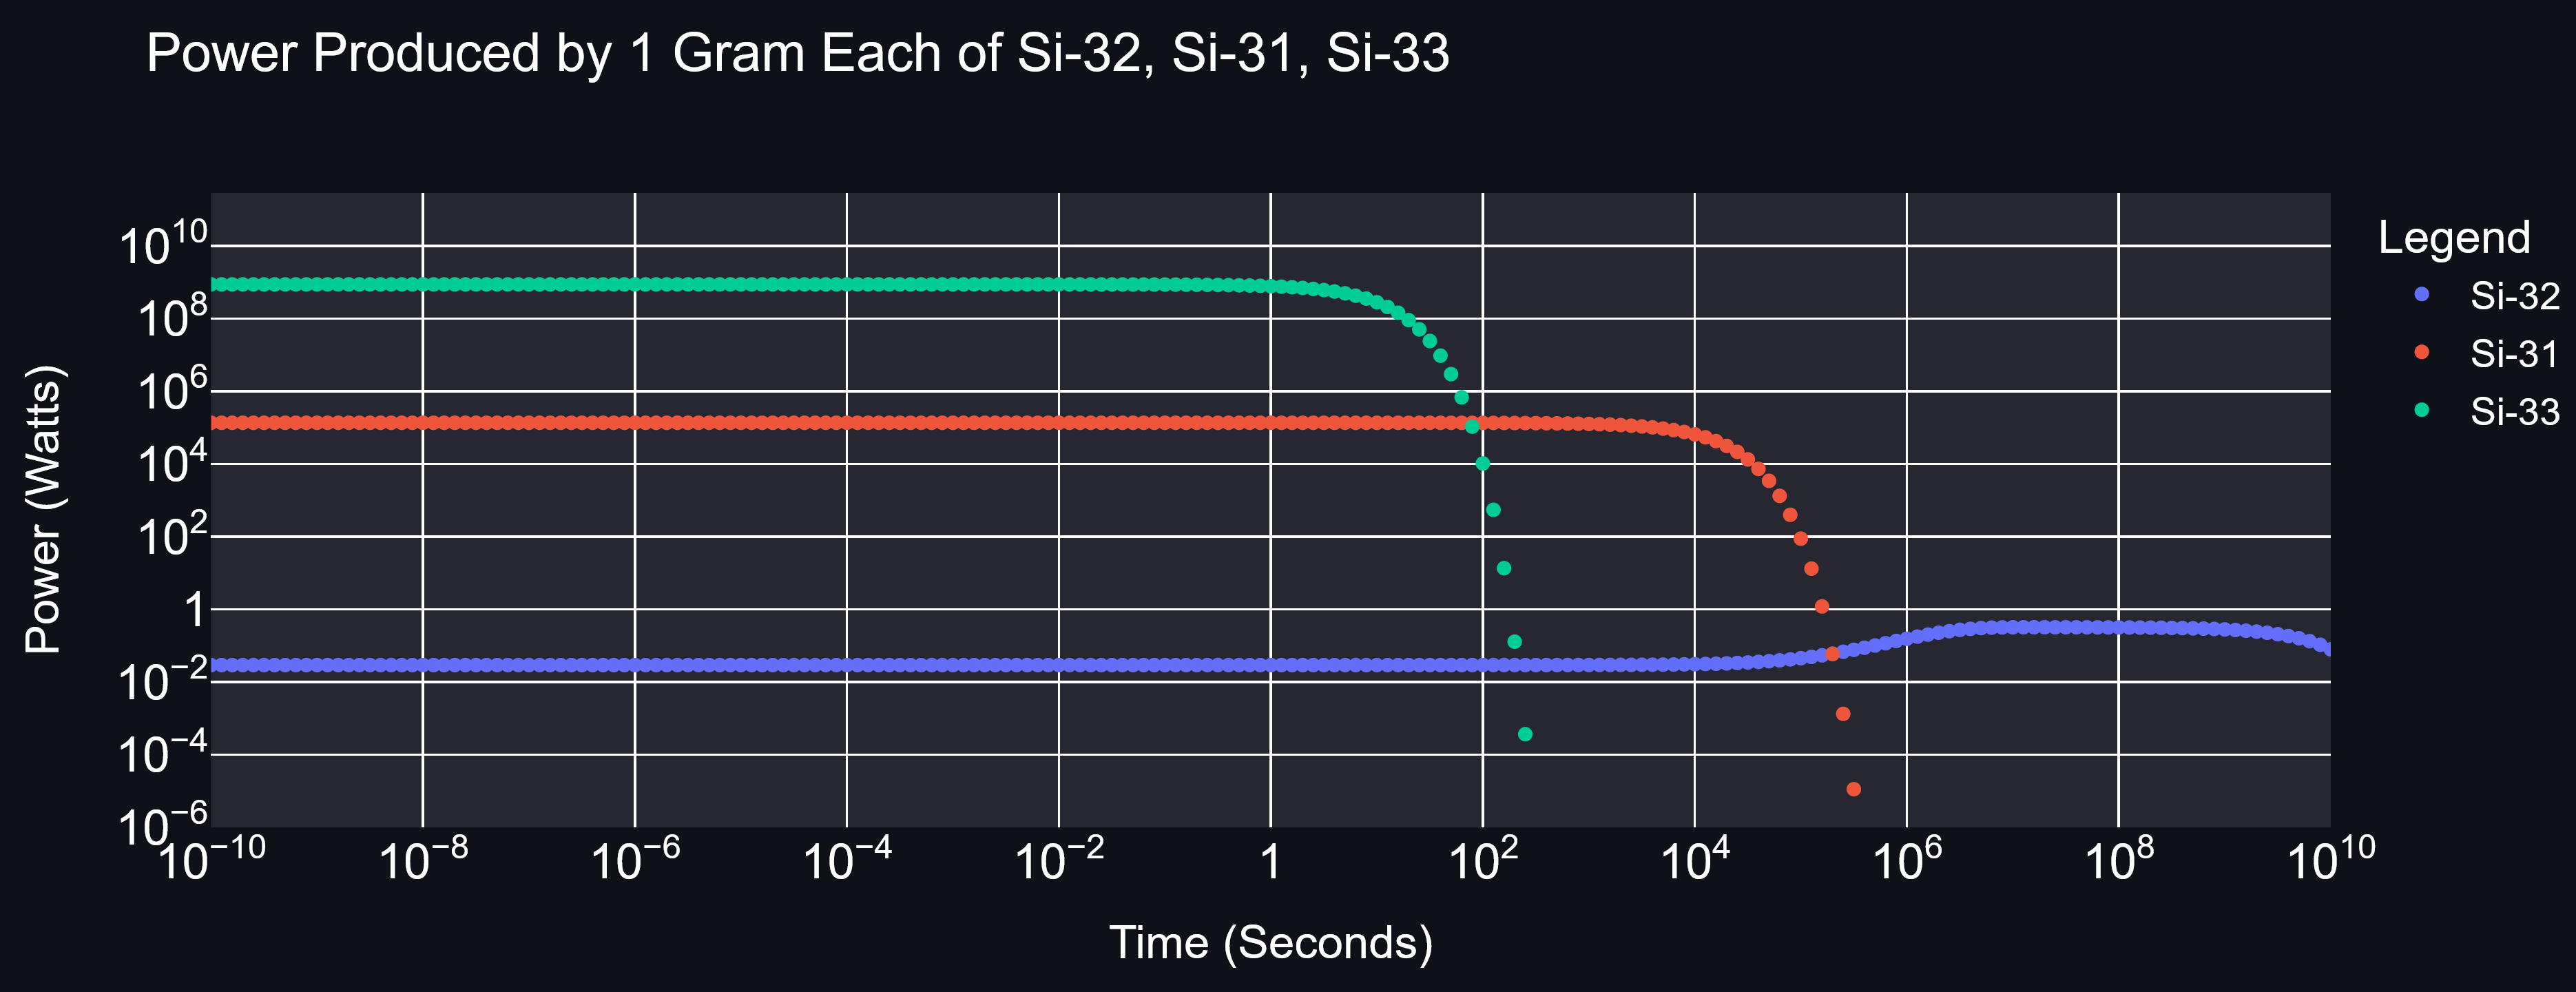
\includegraphics[scale=.65]{Images/silicon_plot.PNG}
\subsubsection{11/19/2022}
Is it possible to produce neutrons for less than 2 MeV each by firing gamma rays into a column of deuterium plasma? How much energy does it take to produce, maintain, and confine the plasma? How could we use the neutrons for nuclear reactions? \\
I calculated the minimum energy it takes to produce neutrons by firing neutrons already obtained a every possible target. What are the same minimum energies for other projectiles? \\
I need to make sure I'm including metastable isotopes as well. Some of them are promising, such as Re-184m. 
\subsubsection{11/20/2022}
Using the same data retrieval methods from the calculations for power released decay chains to analyze metastable isotopes. found over 900 metastable isotopes in ENDF8. Metastable isotopes where the projectile is an electron or gamma ray could be used for rechargable batteries.\\
JENDL5 appears to have more isotopes overall and 71 more metastable isotopes, so I will be using that decay dataset instead. \\
Build format detection software?
\subsubsection{11/21/2022}
By analyzing JENDL5 data and falling back on ENDF8 when necesssary, I have found 89 ground states with half lives longer than 4 months. Now to analyze the stability of excited states, and if they can be used for net energy release. 
\subsubsection{11/22/2022}
The theoretical maximum of the specific energy $\rho_{E,m}$ of a fuel is 
\begin{equation}
    \rho_{E,m} = \frac{E}{M} \cdot \frac{N_A\cdot 1 \text{ eV}}{1 \text{ Joule}} \approx 
    \frac{E}{M} \cdot 10^5 
\end{equation}
where $N_A$ is Avogadro's constant, $E$ is the reaction energy in electronvolts, $M$ is the molar mass in grams, and $\rho_{E,m}$ is in Joules per gram. 
\subsubsection{11/23/2022}
What are the cross sections for nuclear excitation and nuclear de-excitation? Inelastic scattering produces excited states. What are the half-lives of these excited states? JENDL5 only lists several dozen. \\
Using the Nuclear Atlas from Jain et al. in 2015 to get the half lives of different excited states. used pdftotext.com and the PyPDF2 Python package. When specifying utf-8 encoding, the python package appears to have been more effective.
\subsubsection{11/25/2022}
Luckily, I was able copy paste all of the text from the 109 page PDF at once without any programming. Adobe Acrobat PDF reader in the view menu has a button named enable scrolling. Once this is clicked, ctrl+a can select all of the text in a PDF at once, so I just copy pasted it into a text file. 
\subsubsection{11/29/2022}
Nubase 2020 includes some excited states. The first energy level ends with "m" and the second ends with "n", and so on for further energy levels. For instance, the fourth metastable isomer of 121Sn is 121Snq. Silicon 28 has 3 excited states denoted $r$, $i$, and $j$. 
\subsubsection{11/30/2022}
Made a new plot that is publicly uploaded to the internet. It shows the half-lives and decay energies of isotopes that have at least one metastable energy state with a half-life longer than one year. I don't think it includes the ground state. \\
Made a very helpful \href{https://marcosp7635.github.io/plots/Long_Lived_Isomers.html}{plot} that is also \href{https://mp7635plots.web.app/Long_Lived_Isomers.html}{on firebase}\\
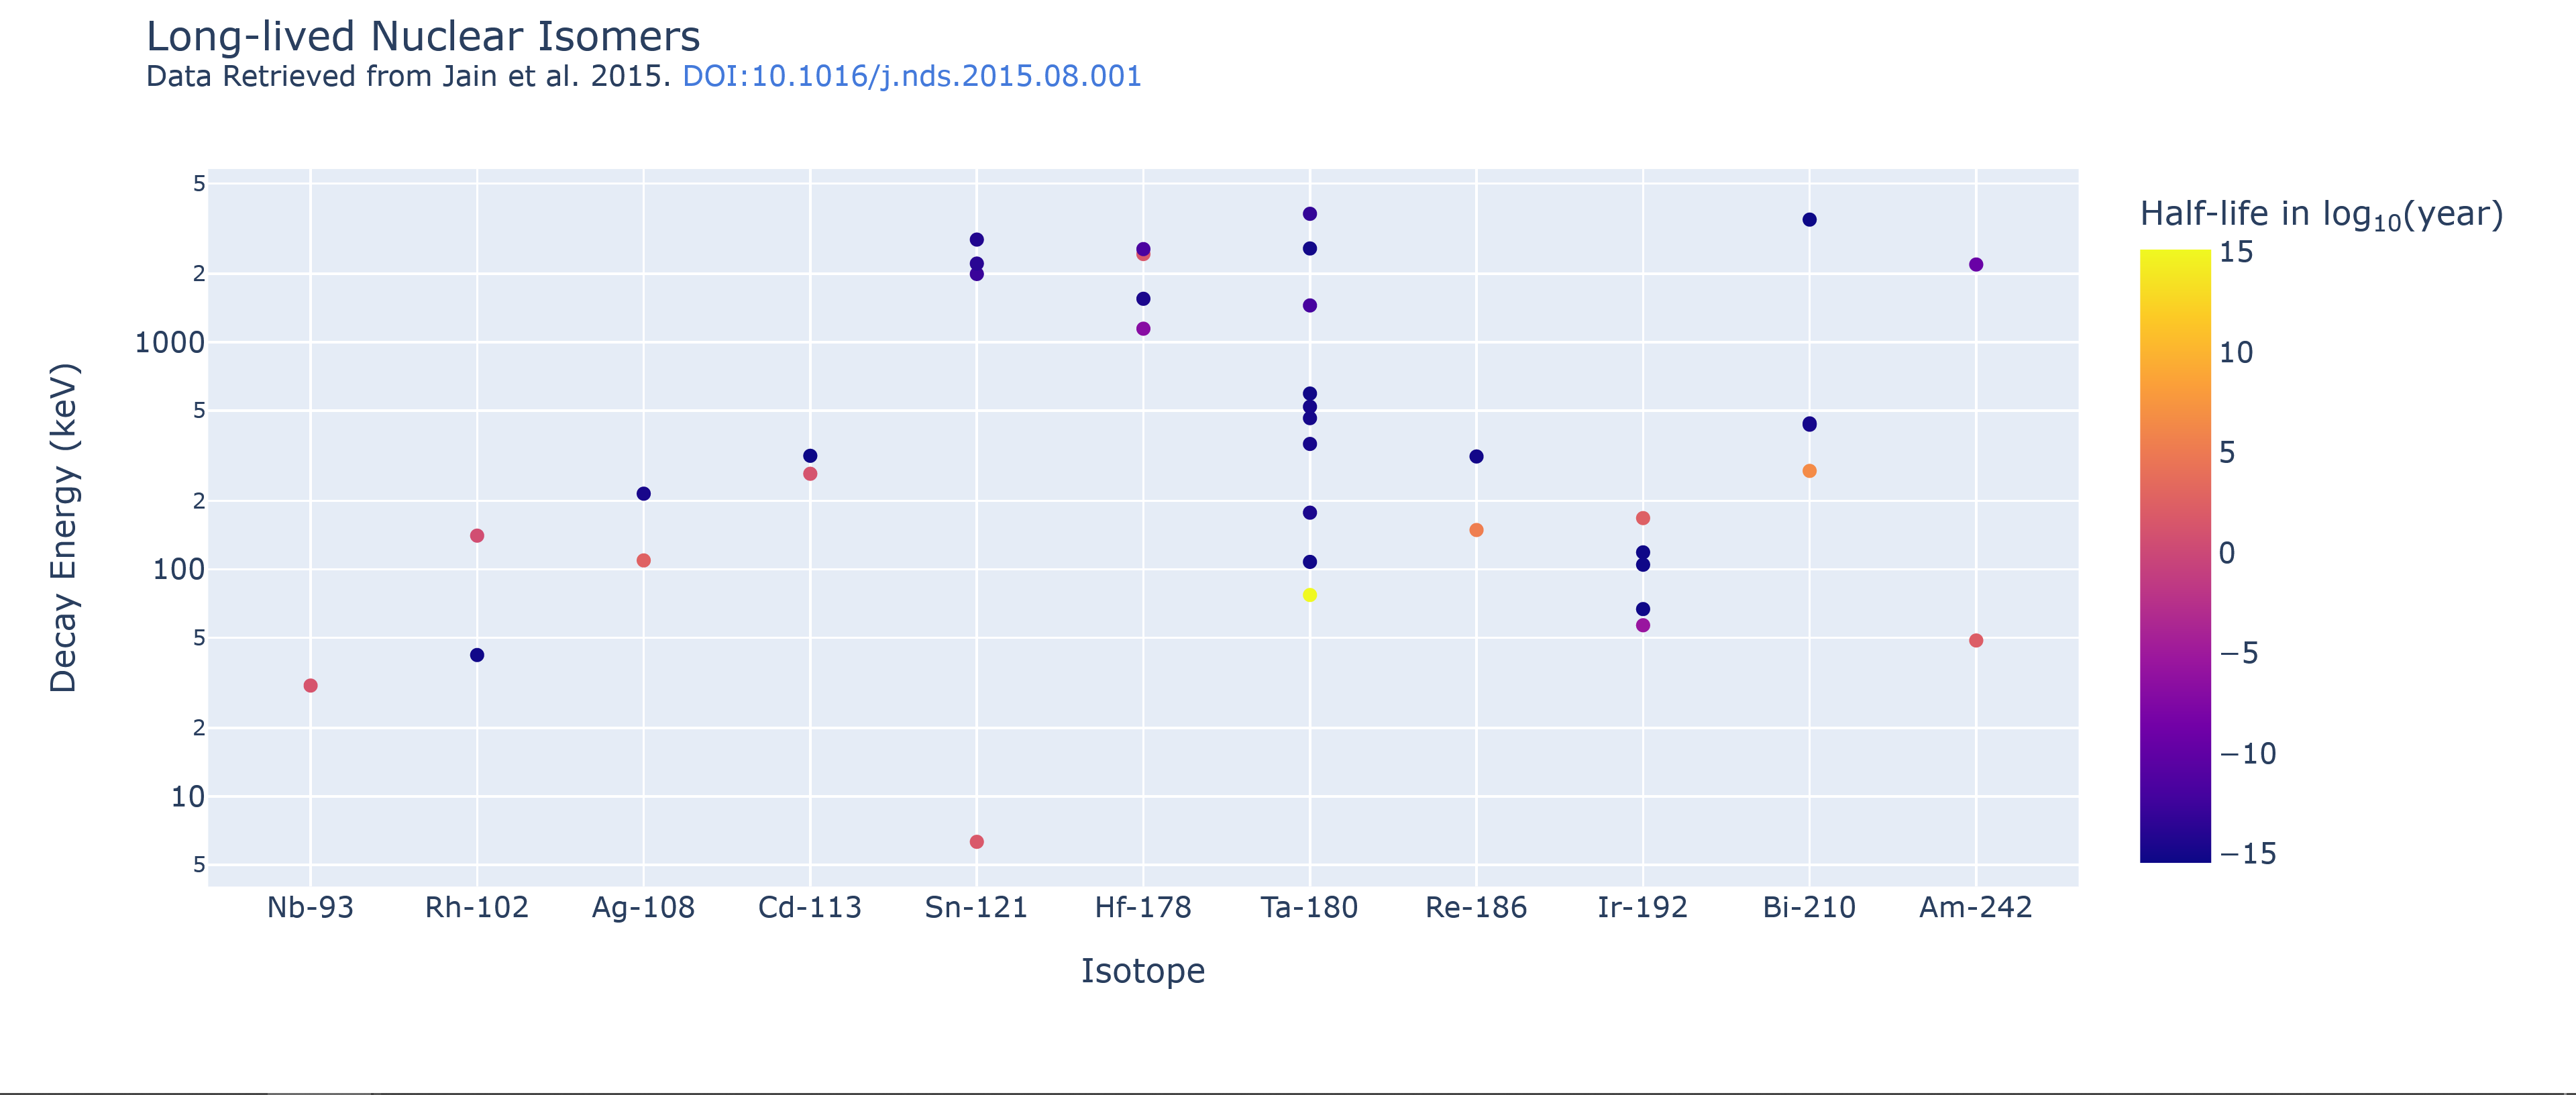
\includegraphics[scale=.65]{Images/helpful_plot.PNG}\\
Thus Hf-178, Ta-180, Ir-192, and Cd-113 seem especially promising.
\section{December}
\subsubsection{12/5/2022}
Since neutrons have a measurable magnetic dipole moment, could a fast beam of neutrons have their kinetic energy directly converted into electricity? This seems possible through Faraday's law of induction. Since 
\begin{equation}\label{eqn:intFaradayLaw}
\begin{split}
\oint_{\partial\Sigma} E \cdot dl = -\frac{d}{dt}\iint_{\Sigma} B \cdot dS
\end{split}
\end{equation}
What is the magnetic flux as a function of the neutron flux? What is the magnetic field from a neutron? I need to make sure to account for relativistic effects. Consider an individual neutron at rest. We have 
\begin{equation}\label{eqn:dipoleB}
\begin{split}
B(r) = \frac{\mu_0}{4\pi}\frac{(3m\cdot\hat{r})\hat{r}-m}{r^3}\\
\text{where $\hat{m}=\hat{r}$ the above line simplifies to} \quad\quad B(r) = \frac{\mu_0}{4\pi}\frac{2m}{r^3}
\end{split}
\end{equation}
where $m$ is the magnetic moment of the neutron, the magnetic field is being measured at a distance $r$ from the neutron, and $\mu_0$ is the vacuum permeability. Since the magnetic moment of the neutron is on the order of $10^{-26}$ J/Tesla, $\mu_0$ is on the order of $10^{-6}$ N/A$^2$, and $4\pi\approx10$ we have 
\begin{equation}
    B\approx r^{-3}\times10^{-33}
\end{equation}
where $r$ is in meters and $B$ is in Teslas. 
\subsubsection{12/6/2022}
Attempting to use GEANT4 on colab and locally installing with wsl. \\
These have been really helpful so far
\begin{lstlisting}[breaklines]
https://www.youtube.com/watch?v=3huHctBp0GE

http://physino.xyz/gears/INSTALL/#install-pre-compiled-geant4-in-windows

https://geant4-userdoc.web.cern.ch/UsersGuides/InstallationGuide/html/postinstall.html#datasets
\end{lstlisting}
\subsubsection{12/7/2022}
Made these interactive maps of research reactors
\href{https://marcosp7635.github.io/plots/reactor_map.html}{github pages version}
\href{https://mp7635plots.web.app/reactor_map.html}{firebase version}
Note that of course the locations are only approximations to show where their host city is on the map. 
\subsubsection{12/14/2022}
Mostly recovered from COVID. I just had an idea\\
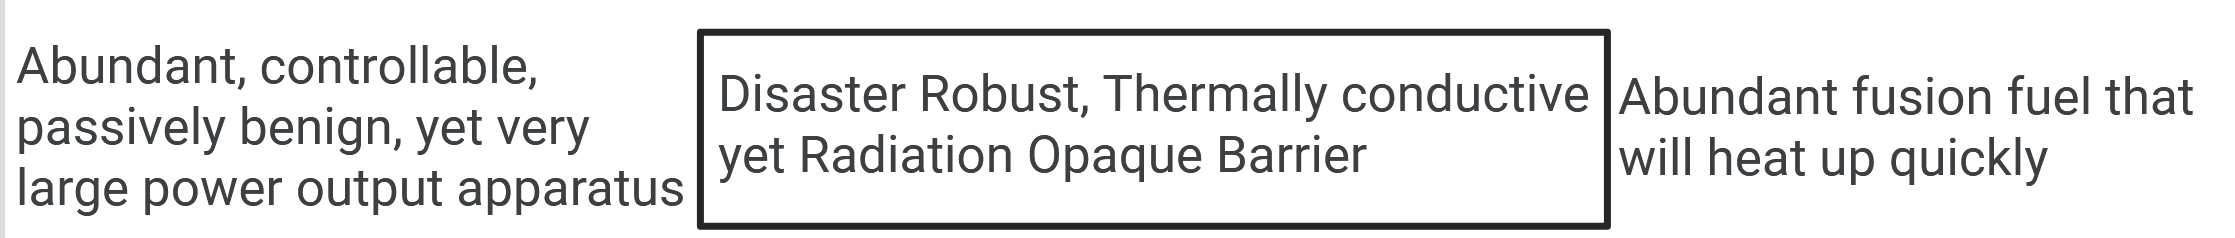
\includegraphics[]{Images/combined_fission_fusion_reactor.PNG}\\
Back to the neutron accelerator, the real $pan \ dulce$ of this operation. 
\subsubsection{12/20/2022}
I forgot that I have a library of empirical data in the subdirectory named exfortables. I will check to see if I have robust Julia code to read the data from it already. \\
solar deuterium neutron source:
Focus sunlight onto beryllium shell of frozen deuterium. The beryllium shell is surrounded by a very thick spherical shell of the neutron target (Hf-178? deuterium? U-238?) which then stores the energy.
\subsubsection{12/26/2022}
General plan for using neutrons for energy efficient nuclear reactions. Since current methods for slowing down neutrons are low throughput, energy production would be needed to offset this process. Thus, using a uranium-powered fission reaction or deuterium (and tritium?) powered fusion reaction to produce both energy and neutrons seems ideal. To slow down high temperature (velocity) neutrons, methods have been developed to study ultracold neutrons by Professor Brad Fillipone and collaborators. I hypothesize that such methods are capable of trapping neutrons into a circular path that can enable a high throughput and incredibly energy efficient nuclear reactions. To see why, consider a formulation for the probability of the occurrence of a given nuclear reaction for an incident neutron
\begin{equation}\label{eqn:RxnProb}
\mathlarger{\text{Probability} = \frac{\sigma\sb{R}}{\sigma\sb{T}}\left(1-e^\mathlarger{\frac{-\sigma\sb{T} \rho x N\sb{A}}{M}}\right)}
\end{equation}
where $\sigma\sb{R}$ is the reaction cross section and $\sigma\sb{T}$ is the total cross section between the target and the incident neutron, and both either have units of barns or m$^{-2}$; $\rho$ is the mass density of the target in kg/m$^3$; $x$ is the path length in m of the neutron through the target; and $M$ is the molar mass of the target in kg/mol; and $N_A$ is Avogadro's constant. One can see that in the limit where 
\begin{equation}\label{eqn:Xlim}
\mathlarger{
x\gg \frac{\sigma\sb{T} \rho N\sb{A}}{M}
}
\end{equation}
which is possible for an incident neutron that makes many trips through the target material as part of a circular neutron accelerator. The result (Equation \ref{eqn:Xlim}) implies that the probability reduces to 
\begin{equation}\label{eqn:Plim}
\mathlarger{
    \text{Probability} = \frac{\sigma\sb{R}}{\sigma\sb{T}}
}
\end{equation}
which would be a revolutionarily efficient nuclear reaction, one that can store great amounts of energy into a small amount of mass, on the order of $10^{6}$ times that of lithium ion batteries using existing radioisotope thermal generators. 
\section{January 2023}
\subsubsection{1/3/2023}
Look into the decay mode of different isomers. For instance, Hf178 gives a maximum energy of 20 times the input energy, however since it is in the form of gamma rays, there in practice this would be closer to 2 times the input energy due to the energy efficiency of currently existing gammavoltaics and thermoelectric devices. Thus, it is worth including the decay mode of different nuclear isomers. \\
Long-lived low specific energy yet incredibly robust and low-maintenance RTGs seem very synergistic with an isomer battery. Specifically, the ability to draw additional power from an isomer battery when needed using the RTG as an input seems very practical. Additionally, the high specific energy of a nuclear isomer based battery would be an ideal method to store energy from an RTG that would otherwise go to waste. 
\subsubsection{1/6/2023}
Emailed a caltech undergrad named sarah who seemed interested in giving the research vc funding were I to found a company. maybe over the summer, and I need to find out what they get in return. \\
What is the gamma ray flux from the Sun in low Earth orbit? Outside the Earth's magnetosphere, it should be measurable. Could the gamma ray flux from the Sun and/or radiation from the Earth's van allen belts be used to produce radioisotopes? Is the flux from both of these source too low such that it would be more efficient to instead use visible light powered particle accelerators or just a ground-based nuclear reactor? \\
How energy efficient would it be to use a proton accelerator to excite Hf-178? Would it be only 1\% efficient? Need to check the cross section for this reaction. 
\subsubsection{1/13/2023}
Using a proton as a projectile to excite Hf-178 nuclei, in order to trap protons in circular orbit with radius $r$ and kinetic energies on the order of 1 MeV, the circular particle accelerator would need to have an electric field on the order of $r$ MV where $r$ is in meters. For safety reasons, what kind of shielding would be necessary and how well contained would the electric field be? What is the cheapest to mass produce the necessary hardware? Is it sustainable and ethical?
\subsubsection{1/22/2023}
For an order of magnitude understanding, how much power would be consumed by a loop of copper wire generating a magnetic field to trap neutrons in a circular path with radius 0.1m? From the Biot-Savart law we have
\begin{equation}
\begin{split}
R = \frac{\rho L}{A}\\
P = I^2R\\
L = 2\pi r\\
B = \mu\sb0I\frac{1}{4\pi r}\\
\end{split}
\end{equation}
where $R$ is the resistance of the wire, $P$ is the power consumed, $\rho$ is the resistivity of the wire material, $L$ is the length of the wire, $r$ is the radius of the circle that the wire circums, and $A$ is the cross sectional area of the wire. By substitution, Equation \ref{eqn:dipoleB}, and solving for $P$ we have \href{https://colab.research.google.com/drive/1OYR0E28cEHTEWVsHOJu20cLt0IZk8A5O?usp=sharing}{https://colab.research.google.com/drive/1OYR0E28cEHTEWVsHOJu20cLt0IZk8A5O?usp=sharing}
\begin{equation}
  P = \frac{8 \pi m^{2} \rho}{A r^{3}} 
\end{equation}
where $m$ is the magnetic dipole moment of the neutron. 
Can we use on-chip step up voltage devices to generate MV electric fields? Can these be used to build particle accelerators for mass production? 
\section{May 2023}
\subsubsection{5/23/2023}
Planning to make a start-up and reach out to labs after final exams in mid-June during SURF. Including notes from this  \href{https://www.youtube.com/watch?v=r-98YRAF1dY&list=PLxpB5Hi17Tp2cAs_OoRZSHqohHJhy9AWo&index=1}{very introductory lecture playlist from Harvard Innovation Labs for startups:}
\\

allow companies and organizations to pay in royalties or pre-paid jobs for high performance teams\\

like the how the water fountains measure the water bottles saved the battery should have a tally of kWh (and Joules and Btu) saved\\

need to find key customers. City-wide power grids for energy storage and back up supplies for hospital

first city-wide power grids. that is slow, so while permitting is happening we should focus on hospitals

also solar farms!

works really really well with solar companies and vehicles
Number 1 priority? which is fast and shows that it works well! probably hospitals, especially in places like puerto rico that struggle with power and solar farms

talk to the solar people about how important storage is

reach out to the user!!!!

remember, the end of knowledge is not the end of answers, but the end of questions
what are we doing?
talking to legal people and business people, then aquire necessary funding (grants, loans, vc, other investors)
You replied to yourself
places that need storage without having access to inclines or lakes
so like the midwest?
you have to be a high priority purchase for the customer, and the only way to know is to ask them
ask them what their number 1 priority is
what would installing this look like? how much would it cost? how long would it take? how would installation inconvenience the existing infrastructure (e.g. something critical like a hospital)?
ask them why wouldn't they buy this product?
let the hospital pay by taking a cut of their profit, and give this profit to the patients
it has to be worth any risk
you need order of magnitude improvement over a crucial problem, which it seems like we have
\section{June 2023}
Can high energy astrophysics data already provide an upperbound on NEEC cross sections? \\
\section{July 2023}
move the target medium instead of the projectile to increase the path length
\section{August 2023}
What reaction cross section and total cross section are needed for a net release of energy from an excited state for a given stopping power? Of course, it would only be net not including the energy it to excite the nucleus.   
\section{September 2023}
Adding more documentation to the neutron production analysis. While looking through the plots in the 
\begin{lstlisting}
Optimized_Radionuclide_Production.ipynb
\end{lstlisting}
file, the tritium production from low energy neutrons impacting Li-6 is surprisingly large from the ENDF8 database, and I mean over 40,000 barns large. How and why is that? 

\section{December 2023}
\subsubsection{Christmas Day}
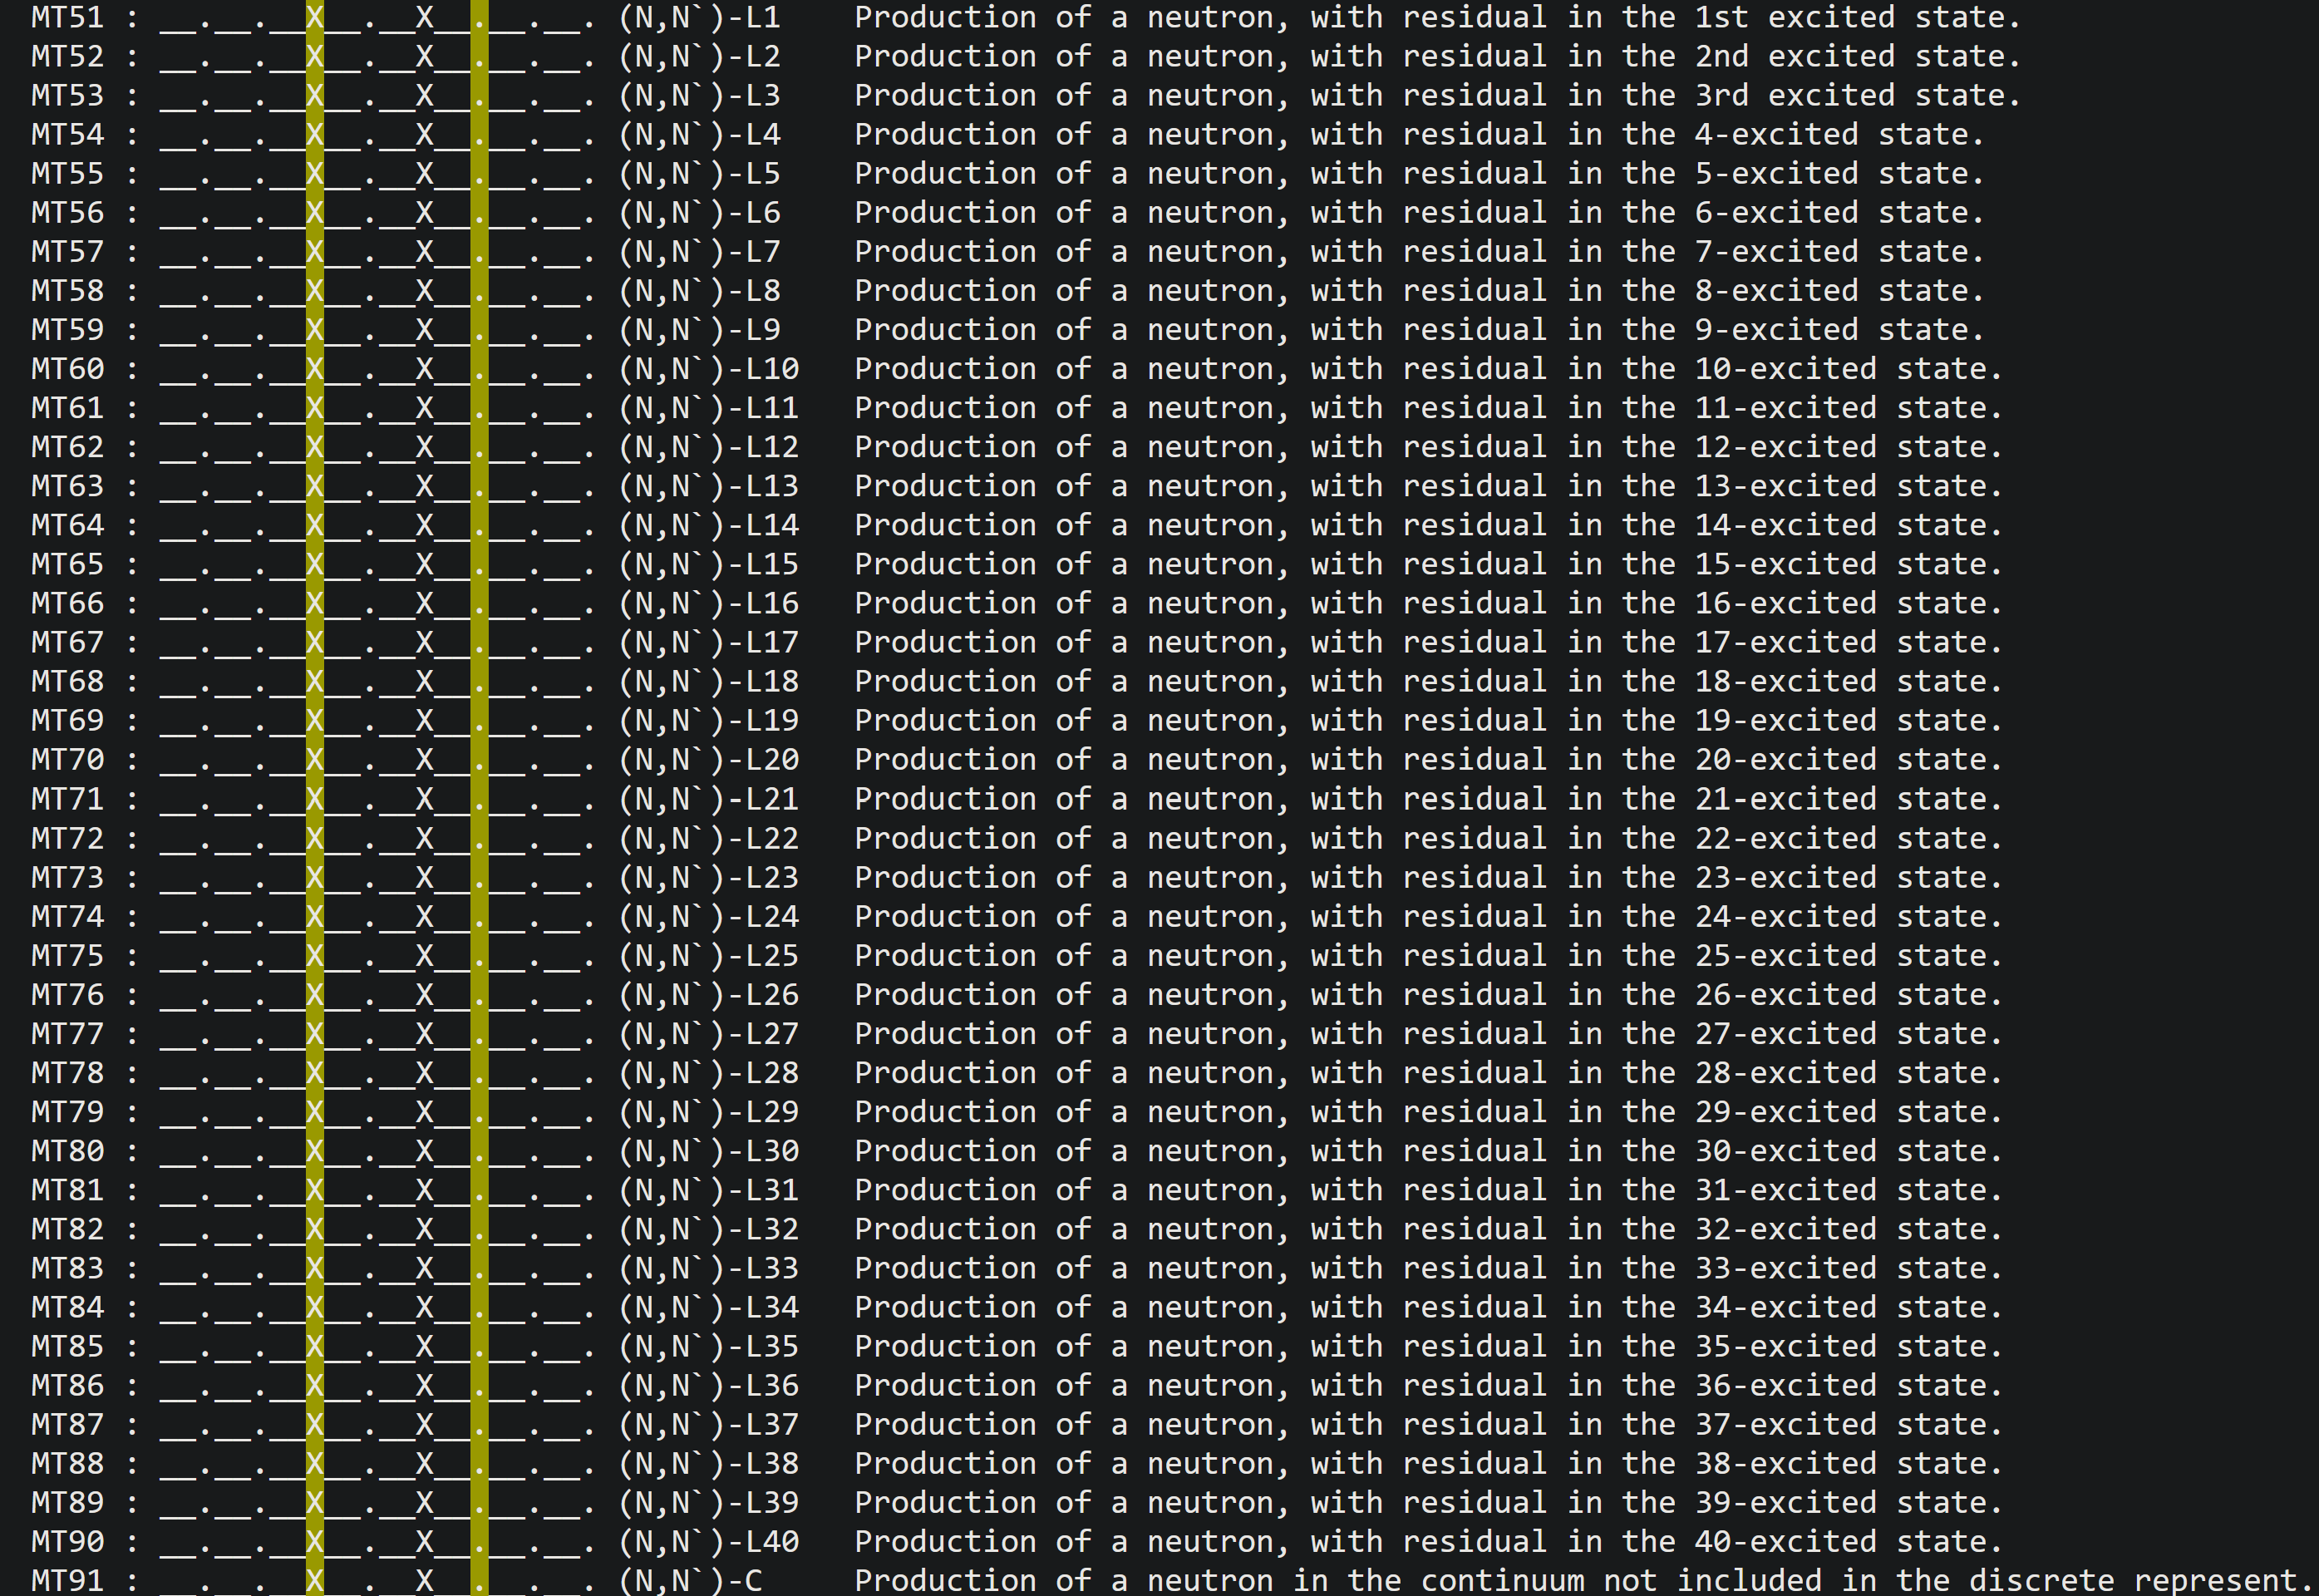
\includegraphics[scale=.7]{Images/excitation_mt_codes_endf_data_explorer.png}\\
What are the criteria for a working energy storage system? What would rigoriously disqualify one? The ratio of the reaction cross section to the total cross section is the upperbound on the efficiency for a given projectile and target, assuming the reaction cross section accounts for all of the possible pathways for energy to be stored.  \\
There is some minimum efficiency that is required for a given isotope's metastable excited states. For energy $E_\text{charged}$ where the isotope is excited from some naturally occurring (ground) state and a higher excited state with energy $E_\text{discharge}$ of the same isotope that has some short half-life, the minimum efficiency, $\mu$ required to merely function as a battery is governed by
\begin{align}
& \mu E_\text{discharge}\ge E_\text{discharge}-E_\text{charged}
\quad\therefore\quad \mu\ge1-\frac{E_\text{charged}}{E_\text{discharge}} 
\end{align}
Thus it is necessary but not sufficient for the reaction and total cross sections $\sigma_\text{reaction}$ and $\sigma_\text{total}$
\begin{align}
\frac{\sigma_\text{reaction}}{\sigma_\text{total}}\ge1-\frac{E_\text{charged}}{E_\text{discharge}} 
\end{align}










\end{document}
